\documentclass{scrartcl}
\usepackage{etex}
\include{header/zusammenfassung}
\include{header/hyperref}
\include{header/listings}
\usepackage{tikz}
\usepackage{adjustbox}
\usetikzlibrary{arrows}
\usetikzlibrary{calc}
\usetikzlibrary{matrix}
\usetikzlibrary{intersections}
\usetikzlibrary{patterns}
\usepackage{pgfplots}
\usepackage{enumitem}

\newcommand\numberthis{\addtocounter{equation}{1}\tag{\theequation}}

\usepackage{longtable}
\usepackage{circuitikz}
\usepackage{esdiff}
\usepackage{textcomp}
\usepackage{float}

\tikzstyle{3x3mask}=[
	matrix of nodes, 
	nodes={draw, minimum size=8mm, anchor=center},
	column sep=0mm
]


% Spaltenabstand bei ,ulticols
\setlength{\columnsep}{1.5em}

\title{OrdDiff Zusammenfassung}
\subtitle{Dozent: A. Henrici - Ordinary Differential Equations}
\author{Ch. Winterhalter, S. Malacarne, H. Diethelm, R. Christen}

\pdfminorversion=6
\raggedbottom

\begin{document}
\selectlanguage{ngerman}

\lstset{language=Matlab}

\maketitle
\tableofcontents
\newpage

\section{Differentialgleichungen}
\[ F(x,y,y',\dots,y^{(n)}) = 0 \]
\textbf{Autonom:} $y' = f(x) \qquad \rightarrow$ nur von $y$ abhängig.\\
\textbf{Explizit:} explizit falls nach $y^{(n)}$ aufgelöst werden kann, ansonsten implizit

\subsection{Lineare homogene autonome DGL 1. Ordnung}

\[ \dfrac{d}{dt}y(t)+ay(t)=0 \qquad y(t_0)=y_0 \]
\begin{tabular}{ll}
Ansatz: & $y(t) = e^{\lambda t}$\\
Einsetzen in DGL: & $\lambda e^{\lambda t} + ae^{\lambda t} = 0$\\
Charakteristisches Polynom: & $\lambda = -a$\\
Allgemeine Lösung: & $y(t) = Ce^{-ax}$\\
\multicolumn{2}{l}{Freiheitsgrad $C$ mit Anfangswert bestimmen} \\
\end{tabular}

\subsection{Lösungsformeln 1. Ordnung}
\subsubsection{Lineare DGL}
\begin{tabular}{p{6cm}p{2cm}p{0.2cm}p{3.8cm}p{6.5cm}}
\textbf{Form:} \quad $y'(x) = f(x) \cdot y(x) + g(x)$ &
\textbf{Vorgehen:} &
1. & $\mu(t)$ berechnen: & $\mu(t) = e^{\int p(t) dt}$ \\ &&
2. & L"osung: & $y(t) = \frac{1}{\mu(t)} \cdot ( \int \mu(t) g(t) dt +c)$ \\ &&
\end{tabular}
Lösung existiert und eindeutig falls $p(t)$ und $g(t)$ stetig.\\
\textbf{Bsp}: $t^3 \cdot y'(t) + 4 t^2 \cdot y(t) = e^{-t} \quad \Longrightarrow \quad y'(t) + \underbrace{4 \frac{1}{t}}_{p(t)} \cdot y(t) = \underbrace{\frac{1}{t^3} e^-t}_{g(t))}$

\subsubsection{Separierbare DGL (wenn autonom, dann auch separierbar)}
\begin{tabular}{p{6cm}p{2cm}p{0.2cm}p{6cm}p{6.5cm}}
\textbf{Form:} \quad $y'(x) = g(x) \cdot h(y)$ &
\textbf{Vorgehen:} &
1.& Gleichung umschreiben: & $\frac{dy}{dx} = g(x) \cdot h(y)$\\ &&
2.& alle $x$-Terme auf die linke Seite: & $\frac{1}{h(y)}dy = g(x) dx$ \\ &&
3.& beide Seiten integrieren: & $\int \frac{1}{h(y)}dy = \int g(x)dx$ \\ & & & & C folgt aus Anf. Bed.\\
\end{tabular} \\
\textbf{Bsp}: $y' = -\frac{x}{y} \Rightarrow \frac{dy}{dx} = -\frac{x}{y} \Rightarrow ydy = -xdx \Rightarrow \int ydy = - \int xdx \Rightarrow \frac{1}{2}y^2 = -\frac{1}{2} x^2 + C$

\subsubsection{Exakte DGL}
\begin{tabular}{p{6.5cm}p{2cm}p{0.2cm}p{3.8cm}p{6.5cm}}
\textbf{Form:} \quad $M(x,y) + N(x,y)\cdot y'(x) = 0$ &
\textbf{Vorgehen:} &
1. & Kompatibilit"ats Bed. pr"ufen: & $\diffp{M(x,y)}{y} = \diffp{N(x,y)}{x}$ \\ &&
2. & $ M(x,y) = \dfrac{d}{dx}\Psi(x,y)$ & $N(x,y) = \dfrac{d}{dy}\Psi(x,y) $ \\ &&
3. & $Q(x,y)$ berechnen: & $Q(x,y) = \int M(x,y) dx$ \\ &&
4. & $\diffp{h(y)}{y}$ berechnen: & $\diffp{h(y)}{y} = N(x,y) - \diffp{Q(x,y)}{y}$ \\ &&
5. & $h(y)$ berechnen: & $h(y) = \int \diffp{h(y)}{y} dy $ \\ &&
6. & L"osung: & $\Psi(x,y) = Q(x,y) + h(y) = c $ \\
\end{tabular} \\
\textbf{Bsp}: $(9x^2 + y -1)dx - (4y -x)dy = 0 \quad \Longrightarrow \quad  \underbrace{9x^2 +y -1}_{M(x,y)} + \underbrace{(-(4y -x))}_{N(x,y)} \cdot \diffp{y}{x} = 0$

\subsubsection{Lösbarkeit}
Eine DGL ist dann lösbar, wenn
\begin{itemize}
	\item 1. Ordnung (DGL oder DGL-System)
	\item eindeutig wenn Anfangswerte gegeben sind
	\item Lipschitz-Stetigkeit erfüllt ist: $\lvert f(t,x_1) - f(t,x_2)\rvert \leq L \lvert x_1 - x_2 \rvert, L = const.$, welche nicht von $y$ abhängt.
\end{itemize}

\subsubsection{Substitution}
\begin{tabular}{p{4cm}p{6cm}}
	$y' = f(ax + by + c)$ & Substitution mit $z = ax + by + c$\\
	& $z = \frac{x}{y}$ und $y' = xz' + z$ \\
\end{tabular}

\subsection{Lineare homogene Differentialgleichung 2. Ordnung}
\begin{tabular}{p{0.25\textwidth}p{0.35\textwidth}p{0.35\textwidth}}
	\multicolumn{3}{l}{\textbf{Lösungsvorgehen:}}\\
	\hline
	DGL:                       		
		& $a \cdot y''(t) + b \cdot y'(t) + c \cdot y(t) = 0$
		&\\
	Allgemeine Lösung:
		& $y(t) = C_1y_1(t) + C_2y_2(t)$
		&\\
	Ansatz:                    		
		& $y_i(t) = e^{\lambda t}$
		&\\
	Charakteristisches Polynom:    	
		& $a\lambda^2 + b\lambda +c =0$
		&\\
	Eigenwerte berechnen:	 		
		& $\lambda_1,\lambda_2 = \frac{-b \pm \sqrt{b^2 - 4ac}}{2a}$
		&\\
	Lösung berechnen:	
		& \multicolumn{2}{l}{Gemäss untenstehender Fallunterscheidung}\\
	Freiheitsgrade:            		
		& \multicolumn{2}{l}{$C_1,C_2$ mit Hilfe der gegebenen Anfangsbedingungen bestimmen.}\\
	\multicolumn{3}{l}{\textbf{Fallunterscheidung der Lösungen:}}\\
	\hline
	Fall 1:                    		
		& $\lambda_1,\lambda_2 \in \mathbb{R}$
		& $y_1(t) = e^{\lambda_1 t}, y_2(t) = e^{\lambda_2 t}$\\
	Fall 2:                    		
		& $\lambda = \lambda_1 = \lambda_2 \And \lambda \in \mathbb{R}$
		& $y_1(t) = e^{\lambda t}, y_2(t) = te^{\lambda t}$\\
	Fall 3:                    		
		& $\lambda_1,\lambda_2 \in \mathbb{C}$
		& $z_1(t) = e^{\lambda_1 t}, z_2(t) = e^{\lambda_2 t}$\\
	    & $y_1(t) = Real(z_1), y_2(t) = Imag(z_1)$\\
	    & oder: $z_{1,2} = a \pm j\beta$
	    & $y_1(t) = e^{ax}\cos(\beta x), y_2(t) = e^{ax} \sin(\beta x)$\\
	\hline
\end{tabular}

$\Rightarrow$ wenn \textbf{$n.$ Ordnung} immer noch ein $\cdot t$ mehr (wie im 2. Fall).\\ 

\subsection{Inhomogen 2. Ordnung}
\begin{tabular}{p{0.4\textwidth}p{0.55\textwidth}}
	\multicolumn{2}{l}{\textbf{Vorgehen:}}\\
	\hline
	1. Homogenes System lösen
		& $a \cdot y''(t) + b \cdot y'(t) + c \cdot y(t) = 0$\\
	2. Inhomogener Ansatz
		& $a \cdot y''(t) + b \cdot y'(t) + c \cdot y(t) = g(t)$\\
	3. $y_s(x)$ in DGL einsetzen.
		&\\
	4. Zusammensetzen
		& $y(t)=y_h(t)+y_p(t)$\\
	\multicolumn{2}{l}{\textbf{Lösungsansätze:}}\\
	\hline
	\multicolumn{2}{l}{
		\begin{tabular}{|p{0.37\textwidth}|p{0.2\textwidth}|p{0.37\textwidth}|}
			\hline
			\textbf{Störfunktion $g(x)$} 	
				& \textbf{Bedingung an $R$}
				& \textbf{Zugehöriger Ansatz für $y_s(x)$} \\
			\hline
			$a$ (const)					 	
				& 
				& $b$ (const) \\ 
			\hline
			$a_0 + a_1x + \dots + a_mx^m$	
				& $0 \in R, n-\mathrm{fach}$
				& $x^n(b_0 + b_1x+ \dots  b_mx^m)$ \\ 
			\hline
			$ae^{\lambda x}$			 	
				& $\lambda \in R, n-\mathrm{fach}$
				& $x^n \cdot be^{\lambda x}$ \\ 
			\hline
			$a \sin(\omega x)$ 					
				&
				& \\
			$b \cos(\omega x)$				 	
				& $\pm j\omega \in R, n-\mathrm{fach}$
				& $x^n(c \sin(\omega x) + d \cos(\omega x))$ \\
			$a \sin(\omega x) + b \cos(\omega x)$ 
				&
				& \\ 
			\hline
		\end{tabular}}\\
\end{tabular}
	
	\vspace{0.5cm}
	
	\textbf{$R$ ist die Lösungsmenge des charakteristischen Polynoms.}
	
\subsection{Variation der Konstanten}
Hat man eine lineare, inhomogene Differentialgleichung 2. Ordnung mit folgender Struktur:\\
\begin{equation*}
y''(t) + p(t)y'(t) + q(t)y(t) = g(t)
\end{equation*}

Um die Variation der Konstanten verwenden zu  können, muss das System in ein System 1. Ordnung gebracht werden:\\
\begin{equation*}
x'(t) = A(t)x(t) + b(t)
\end{equation*}
\begin{equation*}
	\begin{vmatrix} 
	        y'(t)\\ 
	        y''(t)\\   
	\end{vmatrix}
	=
	\begin{vmatrix} 
	        x_1'(t)\\ 
	        x_2'(t)\\   
	\end{vmatrix}
	=
	\begin{vmatrix} 
	        0 && 1\\ 
	       -q(t) && -p(t)\\   
	\end{vmatrix}
	\begin{vmatrix} 
	        x_1(t)\\ 
	        x_2(t)\\   
	\end{vmatrix}
	+
	\begin{vmatrix} 
	        0\\ 
	        g(t)\\   
	\end{vmatrix}
\end{equation*}
In einem ersten Schritt wird die homogene Gleichung gelöst und wir erhalten zwei Fundementallösungen $y_1(t)$ und $y_2(t)$, damit erhalten wir eine Fundamentalmatrix der Form: \\
\begin{equation*}
X(t) = 
	\begin{vmatrix} 
	        y_1(t) && y_2(t)\\ 
	        y_1'(t) && y_2'(t)\\ 
	\end{vmatrix}
\end{equation*}
Um nun die partikuläre Lösung zu erhalten, verwenden wir folgende Gleichung: 
\begin{equation*}
y_P(t) = X(t) \int{X(t)^{-1}b(t)dt}
\end{equation*}
Die gesamte Lösung ergibt sich dann wieder aus der Summe der homogenen sowie der partikulären Lösung. 

\subsubsection{Richtungsfeld und Lösung - Begriff der Lösung}
Die Lösung der Differentialgleichung $\frac{d}{dt}x(t) = f(t,x(t))$ ist eine parametrisierte Kurve x(t). Die Ableitung nach t ist demnach der Tangentenvektor an diese Kurve. Die Diffgleichung enthält demnach die Information über die Tangentenvektoren an ihre Lösungskurven. 
Das bedeutet, auch ohne die Lösung können wir die rechte Seite der Gleichung - d.h. die Tangentenvektoren - zeichnen. Das Lösen der Gleichung ist schlussendlich nur das Einpassen von Kurven in dieses Vektorfeld. Solche Kurven sind die Trajektorien der Gleichung. Die Trajektorie ist jedoch \textbf{nicht} die Lösung, da als Beispiel die Zeitkomponente fehlt. Hätte man (t,x(t)), hätte man die gesamte Lösung.
 
 \vspace{0.5cm}
 
 In \ref{fig:xPrime_x} erkennt man das Verhalten von $\dot{x}$ abhängig von $x$. Diese Erkenntnisse können verwendet werden, um das Richtungsfeld in Abbildung \ref{fig:x_t_quiver} zu zeichnen. Der Wert der Kurve $\dot{x}$ entspricht der Steigung der Pfeile in Abbildung \ref{fig:x_t_quiver}.
 
 \begin{figure}[H]
	\centering
	\begin{subfigure}[h]{0.45\linewidth}
		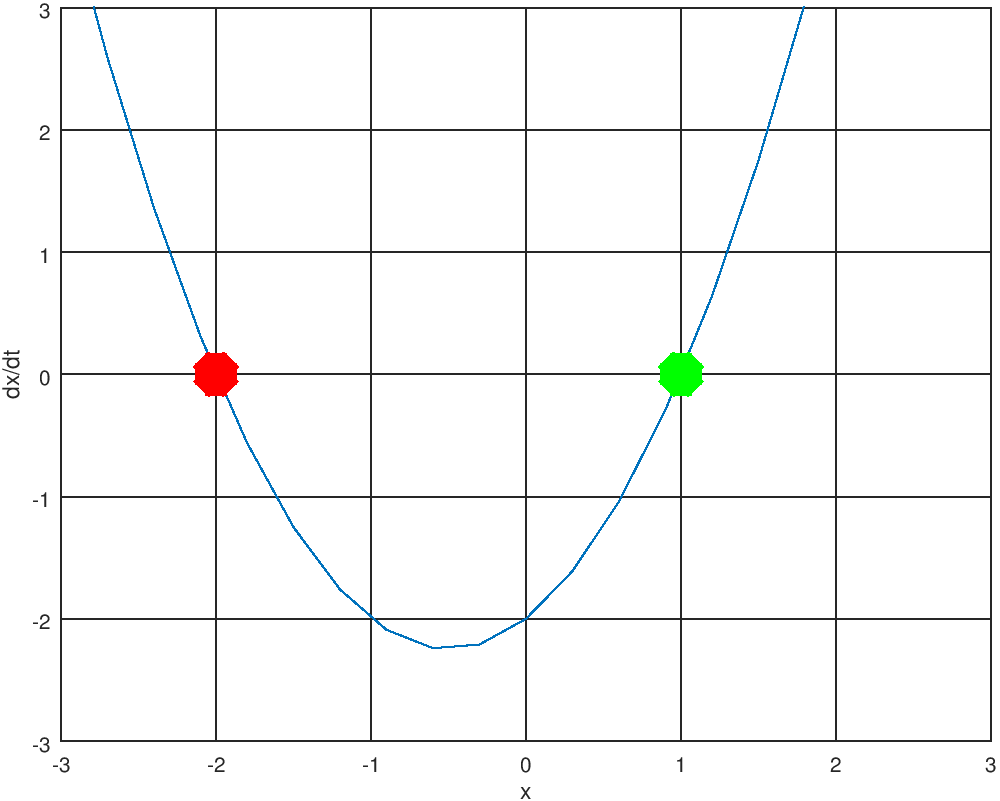
\includegraphics[width=\linewidth]{images/xPrime_x.png}
		\caption{Example plot of $\dot{x} = f(x)$}
		\label{fig:xPrime_x}
	\end{subfigure}
	\begin{subfigure}[h]{0.45\linewidth}
		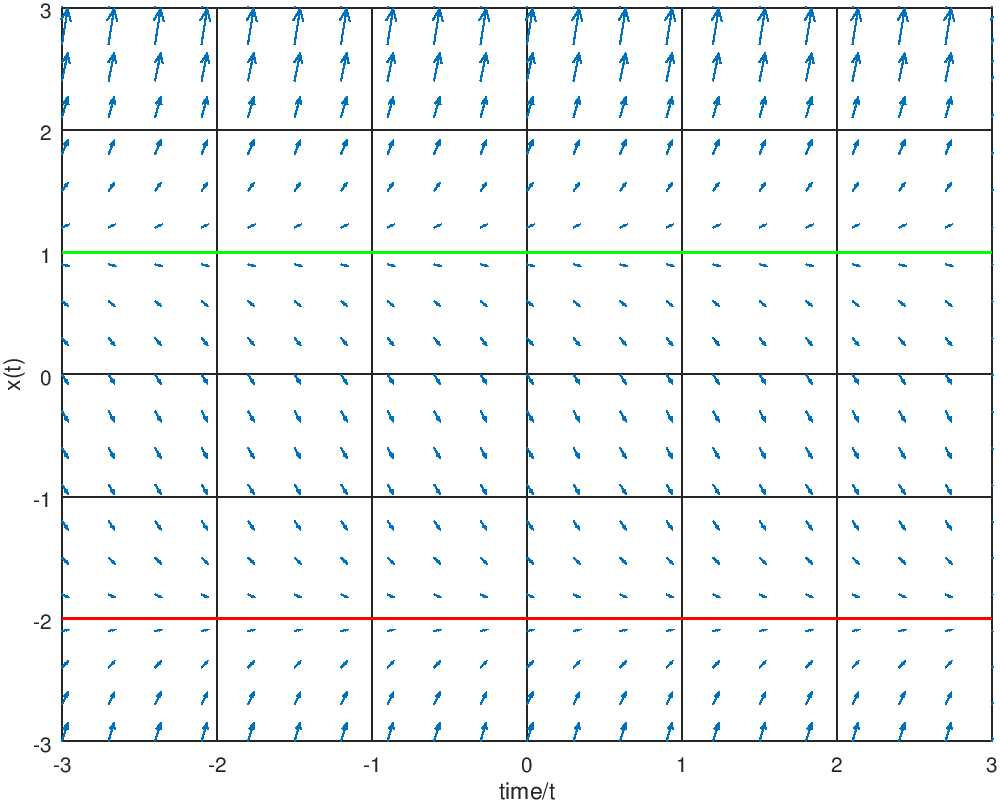
\includegraphics[width=\linewidth]{images/x_t_quiver.png}
		\caption{Corresponding direction field $x(t)$}
		\label{fig:x_t_quiver}
	\end{subfigure}
	\caption{Relationship between the plot of the differential equation and the direction field.}
\end{figure}


\section{Differentialgleichungssysteme}

\subsection{Matrixdarstellung}
Für ein $n$-dimensionales DGL-System 1. Ordnung
\begin{equation*}
    \left.
    \begin{array}{ll}
        x_1'(t) &= f_1(t,x_1(t),\ldots,x_n(t)) \\
        &\hspace{1mm}\vdots \\
        x_n'(t) &= f_n(t,x_1(t),\ldots,x_n(t)) \\
    \end{array}
    \right\}
    x'(t) = f(t,x(t))
    \qquad \text{mit AB} \quad
    \left.
    \begin{array}{ll}
        x_1(t_0) &= x_{1,0} \\
        &\hspace{1mm}\vdots \\
        x_n(t_0) &= x_{n,0} \\
    \end{array}
    \right\}
    x(t_0) = x_0    
\end{equation*}
kann falls \emph{$f$ linear} eine Matrixform aufgestellt werden:
\[ x' = Ax + b \]

Das System is autonom, falls alle $a_{ij}$ konstant und homogen falls alle $b_i=0$.

Kritische Punkte: $x' = Ax + b = 0$, Gleichgewicht: $b = -Ax$ oder $x = -A^{-1}*b$\\
Lösungen bei b=0 (homogenen Gleichung): Für jeden Eigenwert und Eigenvektor eine Lösung: \\
\begin{enumerate}[label=\alph*)]
    \item Ist $\lambda$ ein einfacher reeller Eigenwert von $A$ mit Eigenvektor $\textbf{v}$, so ist die Lösung: $x(t) = C \cdot e^{\lambda t}\textbf{v}$ 
    \item Ist $\lambda$ ein $k$-facher reeler Eigenwert von $A$, so ist die Lösung: \\ \begin{equation*}
    	\textbf{x}_1(t) = C_1 \cdot e^{\lambda t}\textbf{p}_0(t), \quad \textbf{x}_2(t) = C_2 \cdot e^{\lambda t}\textbf{p}_1(t), \quad \dots, \quad \textbf{x}_k(t) = C_k \cdot e^{\lambda t} \textbf{p}_{k-1}(t)
    \end{equation*}
    Falls es nur einen einzigen (linear unabhängigen) Eigenvektor $\textbf{v}$ gibt, muss noch ein \textit{verallgemeinerter Eigenvektor} gefunden werden (wenn 2. Ordnung).
    \begin{equation*}
    	(A - \lambda E_n)\textbf{p}^* = \textbf{v} \Rightarrow (A-\lambda E_n)^2 \textbf{p}^* = 0
    \end{equation*}
    \item Ist $\lambda = \mu + j\nu$ ein einfacher echt komplexer Eigenwert ($\nu \neq 0$) von $A$ und $\textbf{v} = a + jb$ ein Eigenvektor von $A$, so ist die Lösung: \\
    \begin{equation*}
		x(t) = e^{\lambda t}\textbf{v} = e^{(\mu + j\nu)t} \left(a + jb\right)
    \end{equation*}
    \begin{equation*}
    	\textbf{z}_1(t) = \operatorname{Re} (e^{\lambda t \textbf{v}}) = C_1 \cdot e^{\mu t} \left(a \cos(\nu t) - b \sin(\nu t)\right)
    \end{equation*}
	\begin{equation*}
    	\textbf{z}_2(t)= \operatorname{Im} (e^{\lambda t \textbf{v}}) = C_2 \cdot e^{\mu t} \left(a \sin(\nu t) + b \cos(\nu t)\right)
    \end{equation*}
    \item Ist $\lambda = \mu + j\nu$ ein mehrfacher echt komplexer eigenwert von $A$, so müssen Fall b) und c) kombiniert werden.
\end{enumerate}

\subsection{Variation der Konstanten}
Gegeben ist ein lineares, inhomogenes System 1. Ordnung: \\
\begin{equation*}
\frac{d}{dt}x(t) = Ax(t) + b(t) 
\end{equation*}
Als erstes werden die Lösungen der homogenen Gleichung gelöst, wir erhalten für jeden Eigenwert und Eigenvektor eine Lösung: 
$x_1(t) = e^{\lambda_1t}v_1,x_2(t) = e^{\lambda_2t}v_2...x_n(t) = e^{\lambda_nt}v_n$. 
Diese Lösungen ergeben unsere \emph{Fundamentalmatrix}:\\
\begin{equation*}
X(t) = 
	\begin{bmatrix} 
	        x_1(t) && x_2(t) && ... && x_n(t)\\    
	\end{bmatrix}
\end{equation*}

Mit Hilfe der Fundamentalmatrix können wir nun die partikuläre Lösung des Systems bestimmen:\\
\begin{equation*}
y_P(t) = X(t) \int{X(t)^{-1}b(t)dt}
\end{equation*}
Die gesamte Lösung ist nun die Summe der homogenen und der partikulären Lösung $y(t) = y_h(t) + y_p(t)$.


\subsection{Superpositionsprinzip}
Gegeben ist folgendes lineares homogenes Gleichungssystem:
\begin{equation*}
\frac{d}{dt}x(t) = A(t)x(t)
\end{equation*}
Das Superpositionsprinzip sagt, dass die Linearkombination der beiden Lösungen $x_1(t)$ und $x_2(t)$ auch wieder eine Lösung des Differentialgleichungssystems ist. 
\begin{equation*}
	x(t) = c_1 x_1(t) + c_2 x_2(t)
\end{equation*}
Wobei $c_1$ und $c_2$ beliebige Skalare sind. 
Das Prinzip kann auch für Systeme höherer Ordnung verwendet werden. \\

Hier ein \textbf{Beispiel} für eine Differentialgleichung zweiter Ordnung: \\
Gegeben: $t^2y''(t)-4ty'(t)+6y(t)=0$, $t>0$, $y_1(t)=t^2$\\
Gesucht: Eine zweite Lösung $y_2(t)$, so dass ${y_1(t),y_2(t)}$ ein Fundamentalsystem ergeben. \\
Vorgehensweise: \\
\textbf{Schritt 1:}\\
Prüfen, ob $y_1(t)$ wirklich Lösung des Systems ist. \\
\textbf{Schritt 2:}\\
Für die zu bestimmende Lösung $y_2(t)$ kommt folgender Ansatz zum Zug: $y_2(t) = v(t)y_1(t)$.\\
\textbf{Schritt 3:}\\
Ansatz $v(t)y_1(t)$ in Differentialgleichung einsetzen. Die Gleichung so weit es geht umformen und danach nach $v(t)$ auflösen. Wenn $v(t)$ bekannt ist, kann $y_2(t)$ berechnet werden. \\
\textbf{Schritt 4:}\\
Auf Grund der beiden Lösungen, kann die Fundamentalmatrix $Y(t) =
\begin{vmatrix} 
	        y_{1}(t) & y_{2}(t)\\ 
	        y'_{1}(t) & y'_{2}(t)\\   
\end{vmatrix} $ berechnet werden und mit Hilfe der Wronskideterminante geprüft werden, ob die Lösungen linear unabhängig sind ($det(W) \neq 0$). 

\subsection{Lineare Unabhängigkeit}
Die lineare Unabhängigkeit der beiden Lösungen $x_1(t)$ und $x_2(t)$ kann mit Hilfe der \textbf{Wronskideterminante} geprüft werden. 
\begin{equation*}
	W(t) = det[X(t)] =    
	\begin{vmatrix} 
	        x_{11}(t) & x_{12}(t)\\ 
	        x_{21}(t) & x_{22}(t)\\   
	\end{vmatrix}
\end{equation*}
Sind $x_1(t)$ und $x_2(t)$ \textbf{linear unabhängig}, dann gilt $W(t) \neq 0$ für alle $t \in I$. \\
Sind $x_1(t)$ und $x_2(t)$ \textbf{linear abhängig}, dann gilt $W(t) = 0$ für alle $t \in I$. \\
Jede Lösung $\Phi(t)$ kann als Linearkombination eines Fundamentalsystems zweier Lösungen $x_1(t)$ und $x_2(t)$ dargestellt werden. Diese Linearkombination wird als die allgemeine Lösung eines linearen homogenen Systems bezeichnet. \\
\textbf{Theorem von Abel}\\
\begin{equation*}
W(t) = c\cdot e^{\int{\operatorname{trace}(A(t))dt}}
\end{equation*}
Spur einer Matrix = Summe der Hauptdiagonalelemente

\subsection{Fluss eines Vektorfeldes / Matrixexponential}
Für ein AWP $x'(t) = A(t) x(t)$ mit $x(t_0)=x_0$ wird der Fluss $\Phi(t)$ so definiert, dass 
\[ x(t) = \Phi(t) \cdot x_0 \]
Dafür müssen $\Phi'(t) = A(t)\Phi(t)$ und $\Phi(t_0) = E$ erfüllt sein.
Daraus folgt das \emph{Matrixexponential} von $A$:

\[
    \Phi(t) = X(t)X(t_0)^{-1} = e^{At} = \sum\limits_{k=0}^{\infty}\frac{(At)^k}{k!}
\]

Damit hat die Lösung x(t) des Anfangswertproblems $x(0) = x_0$ folgende Form: 
\[
    x(t) = e^{At}x_0
\]


Beispiele:\\
Gegeben: $A = 	\begin{vmatrix} 
	        		\lambda & 0\\ 
	        		0 & \lambda\\   
				\end{vmatrix} 
				\rightarrow$ 
$e^{tA} = \begin{vmatrix} 
	        		e^{t\lambda} & 0\\ 
	        		0 & e^{t\lambda}\\   
				\end{vmatrix}$\\
Gegeben: $A = 	\begin{vmatrix} 
	        		\lambda & 1\\ 
	        		0 & \lambda\\   
				\end{vmatrix} 
				\rightarrow$ 
$e^{tA} = \begin{vmatrix} 
	        		e^{t\lambda} & te^{t\lambda}\\ 
	        		0 & e^{t\lambda}\\   
				\end{vmatrix}$\\
				
Gegeben: $A = 	\begin{vmatrix} 
	        		2 & 3\\ 
	        		3 & 2\\   
				\end{vmatrix} \rightarrow
				\lambda_1=5 \; \lambda_2=-1 \rightarrow ev_1=\begin{vmatrix}
					1\\ 
					1\\   
				\end{vmatrix} \;
				ev_2=\begin{vmatrix}
					1\\ 
					-1\\   
				\end{vmatrix} \rightarrow
				T=\begin{vmatrix} 
	        		1 & 1\\ 
	        		1 & -1\\   
				\end{vmatrix} \rightarrow 
				B=T^{-1} \cdot A \cdot T=\begin{vmatrix} 
	        		5 & 0\\ 
	        		0 & -1\\   
				\end{vmatrix} \rightarrow$\\
				\hspace*{4cm}$e^{tA}=T \cdot e^{tB} \cdot T^{-1}=
				T \cdot \begin{vmatrix} 
					e^{5 t} & 0\\ 
					0 & e^{-t}\\   
				\end{vmatrix} \cdot T^{-1} =
				\dfrac{1}{2}\begin{vmatrix} 
					e^{5 t} + e^{-t}& e^{5 t} - e^{-t}\\ 
					e^{5 t} - e^{-t} & e^{5 t} + e^{-t}\\   
				\end{vmatrix}$

\subsection{Degenerierte Matrizen}
Ist $A$ degeneriert, bedeutet dies, dass sie mindestens einen Eigenwert $\lambda$ mit einer geometrischen Vielfachheit (Anzahl Eigenvektoren) besitzt, die kleiner als seine algebraische Vielfachheit (Anzahl gleiche Eigenwerte $m$) ist. 
Das bedeutet, dass die linear unabhängigen Eigenvektoren der Matrix $A$ den Raum $\mathbb{R}^n$ nicht ausschöpft.\\
Ist $\lambda$ ein Eigenwert von $A$ mit der algebraischen Vielfachheit $m$, dann besitzt die Gleichung: 
\begin{equation*}
(A-\lambda E)^m b_k = 0
\end{equation*}
eine Anzahl $m$ linear unabhängige Lösungen $b_1$ bis $b_m$ und für $k = 1,\ldots,m$ sind die vektorwertigen Funktionen
\begin{equation*}
x_k(t) = e^{\lambda t}\left[{b_k + \frac{t}{1!}(A-\lambda E)b_k + ... + \frac{t^{m-1}}{(m-1)!}(A-\lambda E)^{m-1}b_k}\right]
\end{equation*}
\begin{equation*}
 \Longrightarrow x_k(t) = e^{\lambda t}(b_k + t (A-\lambda E) b_k))
\end{equation*}
linear unabhängige Lösungen der Differentialgleichung. 
\subsection{Beispiel}
Folgende Matrix A ist gegeben: 
\begin{equation*}
	A =     
\begin{bmatrix} %phantom is for spacing
	2 & 0 & -1\\
	0 & 3 & 1\\
	0 & 0 & 2\\
\end{bmatrix}
\end{equation*}
\begin{equation*}
\det(A-\lambda E) = 0 \qquad \Longrightarrow \lambda_1 = 2 \text{(Doppelt)} \quad \lambda_2 = -1
\end{equation*}

\textbf{Schritt 1:} Eigenvektoren berechenen (Hier im Beispiel nur für $\lambda_1$)\\
\begin{equation*}
(A - \lambda_1 E)\nu = 0 \qquad \Longrightarrow \nu = 
\begin{bmatrix} %phantom is for spacing
	1 \\
	0 \\
	0 \\
\end{bmatrix}
\end{equation*}


\begin{equation*}
\Longrightarrow \text{Nur ein Eigenvektor aber zwei Eigenwerte $\lambda_1 = 2$} \quad \Longrightarrow m = 2
\end{equation*}
\textbf{Schritt 2:} Basisvektorern $b_k$ bestimmen \\
\begin{equation*}
(A-\lambda E)^2 b_k = 0 \qquad \Longrightarrow 0\cdot b_{k1} + 9\cdot b_{k2} - 3\cdot b_{k3} = 0
\end{equation*}
\begin{equation*}
b_1= 
\begin{bmatrix} %phantom is for spacing
	1 \\
	0 \\
	0 \\
\end{bmatrix}
\qquad b_2= 
\begin{bmatrix} %phantom is for spacing
	0 \\
	1 \\
	3 \\
\end{bmatrix}
\end{equation*}
\textbf{Schritt 3:} Lösung bestimmen\\
\begin{equation*}
x_1(t) = e^{2 \cdot t} (b_1 + t(A -  2 E)b_1) \qquad \Longrightarrow e^{2\cdot t}
\begin{bmatrix} %phantom is for spacing
	1 \\
	0 \\
	0 \\
\end{bmatrix}
\end{equation*}
\begin{equation*}
x_2(t) = e^{2 \cdot t} (b_2 + t(A -  2  E)b_2) \qquad \Longrightarrow e^{2\cdot t}
\begin{bmatrix} %phantom is for spacing
	-3t \\
	1 \\
	3 \\
\end{bmatrix}
\end{equation*}
\begin{equation*}
 \Longrightarrow X(t) = 
\begin{bmatrix} %phantom is for spacing
	 x_1(t) & x_2(t) \\
\end{bmatrix}
=
\begin{bmatrix} %phantom is for spacing
	1 \cdot e^{2 \cdot t} & -3t \cdot e^{2 \cdot t} \\
	0 & 1\cdot e^{2 \cdot t}  \\
	0 & 3 \cdot e^{2 \cdot t} \\
\end{bmatrix}
\end{equation*}

\subsection{Umwandlung in ein System 1. Ordnung}\label{2to1}
Skalare, lineare, homogene DGL 2. Ordnung mit konstanten Koeffizienten:
\[a \cdot y''(t) + b \cdot y'(t) + c \cdot y(t) = 0 \]
Substitution: \qquad $x_1(t) = y(t) \qquad \text{und} \qquad x_2(t) = y'(t)$\\
\[
	\begin{vmatrix} 
	        y'(t)\\ 
	        y''(t)\\   
	\end{vmatrix}
	=
	\begin{vmatrix} 
	        x_1'(t)\\ 
	        x_2'(t)\\   
	\end{vmatrix}
	=
	\begin{vmatrix} 
	        x_2(t)\\ 
	        -\frac{b}{a} - \frac{c}{a}x_1(t)\\   
	\end{vmatrix}
\]
ergibt das DGL System:\\
\begin{equation*}
x'(t) = Ax(t)
\end{equation*}
\begin{equation*}
	\begin{vmatrix} 
	        x_1'(t)\\ 
	        x_2'(t)\\   
	\end{vmatrix}
	=
	\begin{vmatrix} 
	        0 && 1\\ 
	       -\frac{c}{a} && -\frac{b}{a}\\   
	\end{vmatrix}
	\begin{vmatrix} 
	        x_1(x)\\ 
	        x_2(x)\\   
	\end{vmatrix}
\end{equation*}

Das DGL System kann nun wie ein homogenes, autonomes DGL System 1. Ordnung gelöst werden. Die Lösung für $x_1(t)$ ist geraade die Lösung der DGL 2. Ordnung, weil $x_1(t) = y(t)$, die Lösung $x_2(t)$ kann als Zwischenresultat betrachtet werden. 
Hat das DGL System 2.Ordnung noch eine Störung $g(t)$, so sieht das äquivalente System 1. Ordnung wie folgt aus:\\
\begin{equation*}
x'(t) = Ax(t) + g(t)
\end{equation*}
\begin{equation*}
	\begin{vmatrix} 
	        x_1'(t)\\ 
	        x_2'(t)\\   
	\end{vmatrix}
	=
	\begin{vmatrix} 
	        0 && 1\\ 
	       -\frac{c}{a} && -\frac{b}{a}\\   
	\end{vmatrix}
	\begin{vmatrix} 
	        x_1(t)\\ 
	        x_2(t)\\   
	\end{vmatrix}
	+
	\begin{vmatrix} 
	        0\\ 
	        g(t)\\   
	\end{vmatrix}
\end{equation*}

\paragraph{Transformation 3.Ordnung} $y'''(t) + p(t)y''(t)+q(t)'(t)+r(t)y(t)=g(t)$:\\
\begin{equation*}
	\begin{vmatrix} 
	        x_1(t)\\ 
	        x_2(t)\\
	        x_3(t)   
	\end{vmatrix}
	=
	\begin{vmatrix} 
	        y(t)\\ 
	        y'(t)\\
	        y''(t)   
	\end{vmatrix}
\end{equation*}
\begin{equation*}
	\begin{vmatrix} 
	        x_1'(t)\\ 
	        x_2'(t)\\
	        x_3'(t)   
	\end{vmatrix}
	=
	\begin{vmatrix} 
	        0 && 1 && 0\\ 
	        0 && 0 && 1\\
	        -r(t) && -q(t) && -p(t)   
	\end{vmatrix}
		\begin{vmatrix} 
		        x_1(t)\\ 
		        x_2(t)\\
		        x_3(t)   
		\end{vmatrix}
		+
			\begin{vmatrix} 
			        0)\\ 
			        0\\
			        g(t)   
			\end{vmatrix}
\end{equation*}

\subsection{Zweite Lösung finden für DGL 2. Ordnung}
Gegeben: Diffgleichung 2. Ordnung mit Lösung, suche eine zweite Lösung.\\
Vorgehen:\\
1. Prüfe, ob erste Lösung $y_1(t)=t^2$ für $t^2y''(t) -4ty(t) +6y(t) = 0$ wirklich Lösung ist. \\
2. Ansatz $y_2(t)=v(t)\cdot y_1(t)$ in DGL einsetzen. \\
3. $v''(t),v'(t),v(t)$ ordnen und $v(t)$ berechnen. \\
4. $y_2(t)=v(t)\cdot y_1(t)$ berechnen und prüfen, obs stimmt.\\
5. Fundamentalmatrix $Y(t) = 	\begin{vmatrix} 
	        						y_1(t) && y_2(t)\\ 
	        						y_1'(t) && y_2'(t)\\ 
								\end{vmatrix}$
berechnen und Wronskideterminante prüfen. 


\subsection{Verschiedene Lösungsansätze für inhomogene lineare Systeme }
\subsubsection{Elimination einer Variablen}

Gegenteil von \ref{2to1}. Aus zwei 1. Ordnungen wird eine 2. Ordnung. Nicht sehr elegant, je nachdem aber sehr effektiv. Anschliessend wie für 2. Ordnung rechnen.

\subsubsection{Entkoppeln}
\begin{equation*}
	A = TDT^{-1} 
\end{equation*}
\begin{equation*}
	D = \mathrm{diag}(\lambda_1, \lambda_2, \dots, \lambda_n)
\end{equation*}
\begin{equation*}
	T = (v_1, v_2, \dots, v_n)
\end{equation*}
\begin{equation*}
	\dot{x} = Ax \rightarrow \dot{x} = TDT^{-1}x \Rightarrow T^{-1}\dot{x} = DT^{-1}x \rightarrow y = T^{-1}x \Rightarrow x = Ty
\end{equation*}

\subsubsection{Verwendung von Matrix-Exponentialen/Variation der Konstanten}
\begin{equation*}
	e^{At} = E_n + At + \frac{A^2t^2}{2!} + \frac{A^3t^3}{3!} + \dots = \sum_{k = 1}^{\infty} A^k \frac{t^k}{k!}
\end{equation*}
\begin{equation*}
	x(t) = \underbrace{e^{At} \int_{0}^{t} e^{-As}b(s)}_{x_s} + \underbrace{e^{At}C}_{x_h}, \qquad C \in \mathbb{R}^n
\end{equation*}
Diese Variante ist sehr elegant, auf Grund der Matrix-Exponential sehr aufwändig.
\subsection{Schwingungen}

\begin{tabular}{|l|l|}
	\hline
	\textbf{Terminologie}              & \textbf{Gleichung} \\ \hline
	freie ungedämpfte Schwingung       & $m \cdot y''(t) + k \cdot y(t) = 0$ \\ \hline
	freie gedämpfte Schwingung         & $m \cdot y''(t) + \gamma\cdot y'(t) + k \cdot y(t) = 0$ \\ \hline
	erzwungene ungedämpfte Schwingung  & $m \cdot y''(t) + k \cdot y(t) = F(t)$ \\ \hline
	erzwungene gedämpfte Schwingung    & $m \cdot y''(t) + \gamma\cdot y'(t) + k \cdot y(t) = F(t)$ \\ \hline
\end{tabular}\\

\textbf{Matrixschreibweise}\\
$ y''(t) + p(t)\cdot y'(t) + q(t) \cdot y(t) = g(t) \rightarrow x' = A \cdot x + b \quad 
A(t)=\begin{bmatrix}
 0 & 1 \\
 -q(t) & -p(t)\\
\end{bmatrix} \quad
b(t)=\begin{bmatrix}
 0 \\
 g(t)\\
\end{bmatrix}$

\textbf{Physikalische Schreibweise}\\
$y'' + 2 \delta y' + \omega_0^2 y = f(t) \qquad \delta = \frac{\gamma}{2 \cdot m} \qquad \omega_0^2 = \frac{k}{m} \qquad f(t) = \frac{F(t)}{m}$ \\

\textbf{Eigenmodi}\\
$C_1 = C_2 = 0 \qquad$ oder $\qquad C_3 = C_4 = 0$\\

\textbf{Dämpfung}\\
Wenn Realteile der Eigenwerte negativ sind, so ist das System gedämpft.
\subsubsection{Freie Schwingung}
$m \cdot y''(t) + \gamma\cdot y'(t) + k \cdot y(t) = 0$\\
\begin{tabbing}
ohne Dämpfung ($\gamma = 0$): \= $y(t) = A \cdot \cos(w_0 \cdot t) + B\cdot \sin(w_0 \cdot t) \qquad w_0=\sqrt{\dfrac{k}{m}} \qquad  A=y_0 \qquad B=\dfrac{y_0'}{w_0}$\\
\>$y(t) =R\cdot \cos(w_0 \cdot t - \varphi) \quad R=\sqrt{A^2+B^2} \quad \varphi=\operatorname{atan2}(B,A)$\\
\end{tabbing}

\begin{tabbing}
mit Dämpfung ($\gamma \neq 0$): \= $Z(\lambda)=m\lambda^2 + \gamma \lambda + k \rightarrow \lambda_{1,2}=\dfrac{-\gamma \pm \sqrt{\gamma^2 - 4 \, m \, k}}{2 \, m} \rightarrow D=\gamma^2 - 4 \, m \, k$\\
\> Fall 1: $D>0 \quad y(t)=Ae^{\lambda_1 \, t} + Be^{\lambda_2 \, t}$\\
\> Fall 2: $D=0 \quad y(t)=(A + B \,t)e^{\lambda \, t}$\\
\> Fall 3: $D<0 \quad y(t)=Ae^{\mu \, t}\cos(\nu \, t) + Be^{\mu \, t}\sin(\nu \, t) \quad \mu=-\dfrac{\gamma}{2\,m} \quad \nu = \sqrt{\dfrac{k}{m}-\dfrac{\gamma^2}{4 \, m^2}}$
\end{tabbing}

$\operatorname{atan2}(B, A) = \begin{cases}
\arctan\left(\frac B A\right) & \qquad A > 0 \\
\arctan\left(\frac B A\right) + \pi& \qquad B \ge 0 , A < 0 \\
\arctan\left(\frac B A\right) + 2\pi& \qquad B < 0 , A < 0 \\
+\dfrac{\pi}{2} & \qquad B > 0 , A = 0 \\
+\dfrac{3\pi}{2} & \qquad B < 0 , A = 0 \\
\text{undefined} & \qquad B = 0, A = 0
\end{cases}$

\subsubsection{Erzwungene Schwingung}
$m \cdot y''(t) + \gamma\cdot y'(t) + k \cdot y(t) = f(t)=Ae^{i\,w\,t} \rightarrow$\\
$ y''(t) + 2 \, \delta y'(t) + w_0^2 \, y(t) = F(t)$ \qquad mit \quad $w_0=\sqrt{\dfrac{k}{m}} \qquad \delta=\dfrac{\gamma}{2\,m} \qquad F(t)=\dfrac{f(t)}{m}$\\
$\rightarrow y(t)=y_h(t)+y_p(t)$

\begin{tabbing}
ohne Dämpfung ($\delta = 0$): \= $y(t) = \dfrac{A}{w_0^2-w^2}(\cos(w_0\,t)-\cos(w\,t))$\\
\> $y(t) = \dfrac{A}{w_0^2-w^2}\sin(\dfrac{w_0-w}{2} \cdot t)\sin(\dfrac{w_0+w}{2} \cdot t)$\\
\end{tabbing}

\begin{tabbing}
mit Dämpfung ($\delta \neq 0$): \= $y_h(t \rightarrow \infty) = 0$\\
\> $y_p(t)= \operatorname{Real}\left(\dfrac{1}{w_0^2-w^2 + 2\,i\,\delta\,w}Ae^{i\,w\,t}\right)$\\
\> $y_p(t)= g(w)\,A\,\cos(wt-\varphi(w))$\\
\> $g(w)=\dfrac{1}{\sqrt{(w_0^2-w^2)^2+4\delta^2w^2}} \quad \varphi(w)=\arccos(\dfrac{w_0^2-w^2}{\sqrt{(w_0^2-w^2)^2+4\delta^2w^2}})$\\
\> $g_{max}=\dfrac{1}{2\delta} \dfrac{1}{\sqrt{w_0^2-\delta^2}}$ bei $w_{max}=\sqrt{w_0^2-2\,\delta^2}$
\end{tabbing}
\begin{minipage}[h]{0.5\textwidth} 
	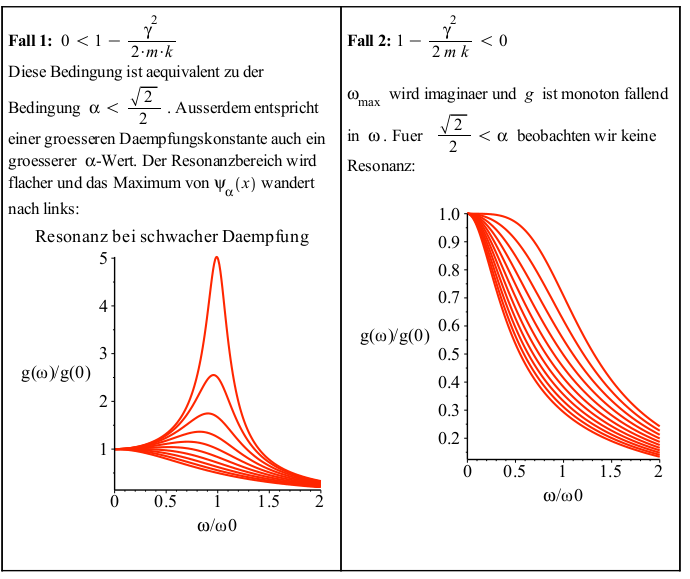
\includegraphics[width=1.0\textwidth]{images/Erzwungen1.png}
\end{minipage}
\begin{minipage}[h]{0.5\textwidth}
	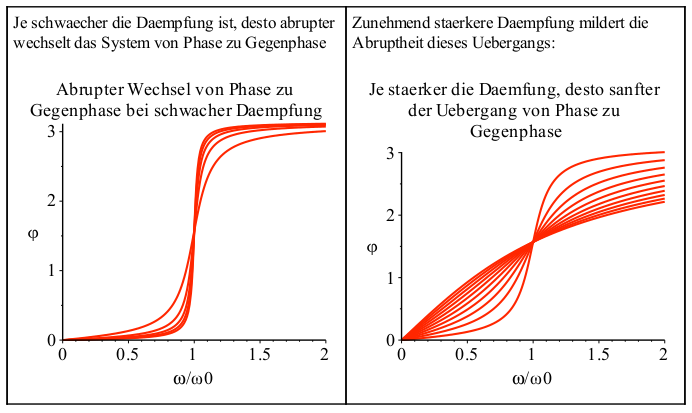
\includegraphics[width=1.0\textwidth]{images/Erzwungen2.png}
\end{minipage}

\subsection{Steife Systeme}
$	\lvert\frac{\lambda_1}{\lambda_2}\rvert \gg 1 \rightarrow \mathrm{impliziter Euler}$


\section{Numerische Verfahren}

\subsection{Fehler}

\begin{tabular}{ll}
Tatsächlicher Wert \quad  & $\phi(t_n)$ \\
Globaler Fehler & $E_n = \smash{\displaystyle\max_{0 \leq k \leq n}} \lvert e_k \rvert = \smash{\displaystyle\max_{0 \leq k \leq n}}\lvert x(t_k) - x_k\rvert$ \\ \\
Lokaler Fehler & $\tau_{k,h} = \frac{x(t_{k+1}) - x_h(t_{k+1}; t_k, x(t_k))}{h}$ \\
Rundungsfehler & $R_n = y_n - Y_n$\, ,\quad wobei $Y_n$ gerundet \\
Lipschitz-Bedingung & $\lvert f(t, x_1) - f(t, x_2)\rvert \leq L \lvert x_1 - x_2 \rvert$ wobei $\dot{x} = f(t,x), L = const.$ \\
\end{tabular}\\ \\
Zwei Lösungen $x^{(1)}(t), x^{(2)}(t)$ bezüglich der Anfangsbedingungen $x_1, x_2$. Dann gilt für alle $t$ in einer Umgebung von $t_0$ die Abschätzung: $\lvert x^{(1)}(t) - x^{(2)}(t)\rvert \leq e^{L(t-t_0)} \lvert x_1 - x_2\rvert $ \newline

\begin{minipage}{0.6\linewidth}
    \subsection{Explizites Euler-Verfahren (Polygonzugmethode)}
    Polygonzug mit Steigung $y'(t)$ und Zeitschritt $h$\\
    $\dot{x} = f(t,x)$ \\
    $t_k = t_0 + k \cdot h$ \\
    $x_{k+1} = x_k + h \cdot f(t_k, x_k)$ \\
    $x_0 = x(0)$ \\
    $|\phi''(t)|<M \qquad |e_n| < \dfrac{M*h^2}{2} \qquad
    h_n < \sqrt{\dfrac{2\epsilon}{M}} \qquad E_n \approx h$\\
    $e_{n+1} = \dfrac{1}{2} \cdot \varphi''(\tau_n)\cdot h^2 \qquad \tau_n \text{ zwischenschritt in } [t_n,t_{n+1}]$\\
    $\varphi''(t)=f_t(t,\varphi(t)) + f_y(t,\varphi(t))\cdot\varphi'(t)$\\\\
\end{minipage}
\begin{minipage}{0.4\linewidth}
  %  \centering
    \begin{tikzpicture}

\begin{axis} [
    clip=false,
    width=8cm, height=4cm,
    axis lines=left,
    domain=-2:2, samples=31,
    ymin=0, ymax=6,
    xmin=-2, xmax=3,
    xticklabels={{},{},{$t_0$},{$t_1$},{$t_2$},{$t_3$},{}},
    yticklabels={},
]
    \node at (axis cs:3.2,0) {$t$};
    \node at (axis cs:-2,6.5) {$y$};
    
    % Plot parabola
    \addplot[HSRBlue,mark=none] {4-0.5*x^2};
    \addplot[HSRBlue,mark=o,only marks,samples=3,domain=-1:1] {4-0.5*x^2};
    
    % p0
    \addplot[black,mark=none,domain=-1.5:-0.5,samples=2] {4.5+x};
    \node[anchor=south] at (axis cs:-1,3.5) {$p_0$};
    \addplot[black,dashed,mark=none,domain=-0.5:0,samples=2] {4.5+x};

    % p1
    \addplot[black,mark=none,domain=-0.5:0.5,samples=2] {4.5};
    \node[anchor=south] at (axis cs:0,4.5) {$p_1$};
    \addplot[black,mark=o] coordinates{(0,4.5)};
    \addplot[black,dashed,mark=none,domain=0.5:1,samples=2] {4.5};
    
    % p2
    \addplot[black,mark=none,domain=0.5:1.5,samples=2] {5.5-x};
    \node[anchor=south] at (axis cs:1,4.5) {$p_2$};
    \addplot[black,mark=o] coordinates{(1,4.5)};
    \addplot[black,dashed,mark=none,domain=1.5:2,samples=2] {5.5-x};
    
    % p3
    \node[anchor=south] at (axis cs:2,3.5) {$p_3$};
    \addplot[black,mark=o] coordinates{(2,3.5)};
    
\end{axis}

\end{tikzpicture}
\end{minipage} 

\begin{minipage}{0.6\linewidth}
    \subsection{Mittelpunktsregel, Polygonzugmethode}
     Modifiziertes Euler-Verfahren mit Schätzung in der Mitte. \\
     $t_k = t_0 + k \cdot h$ \\
     $x_{k+\frac{1}{2}} = x_k + \frac{h}{2} \cdot f(t_k, x_k)$ \\
     $x_{k+1} = x_k + h \cdot f(t_k + \frac{h}{2}, x_{k+\frac{1}{2}})$ \\
\end{minipage}
\begin{minipage}{0.4\linewidth}
   % \centering
	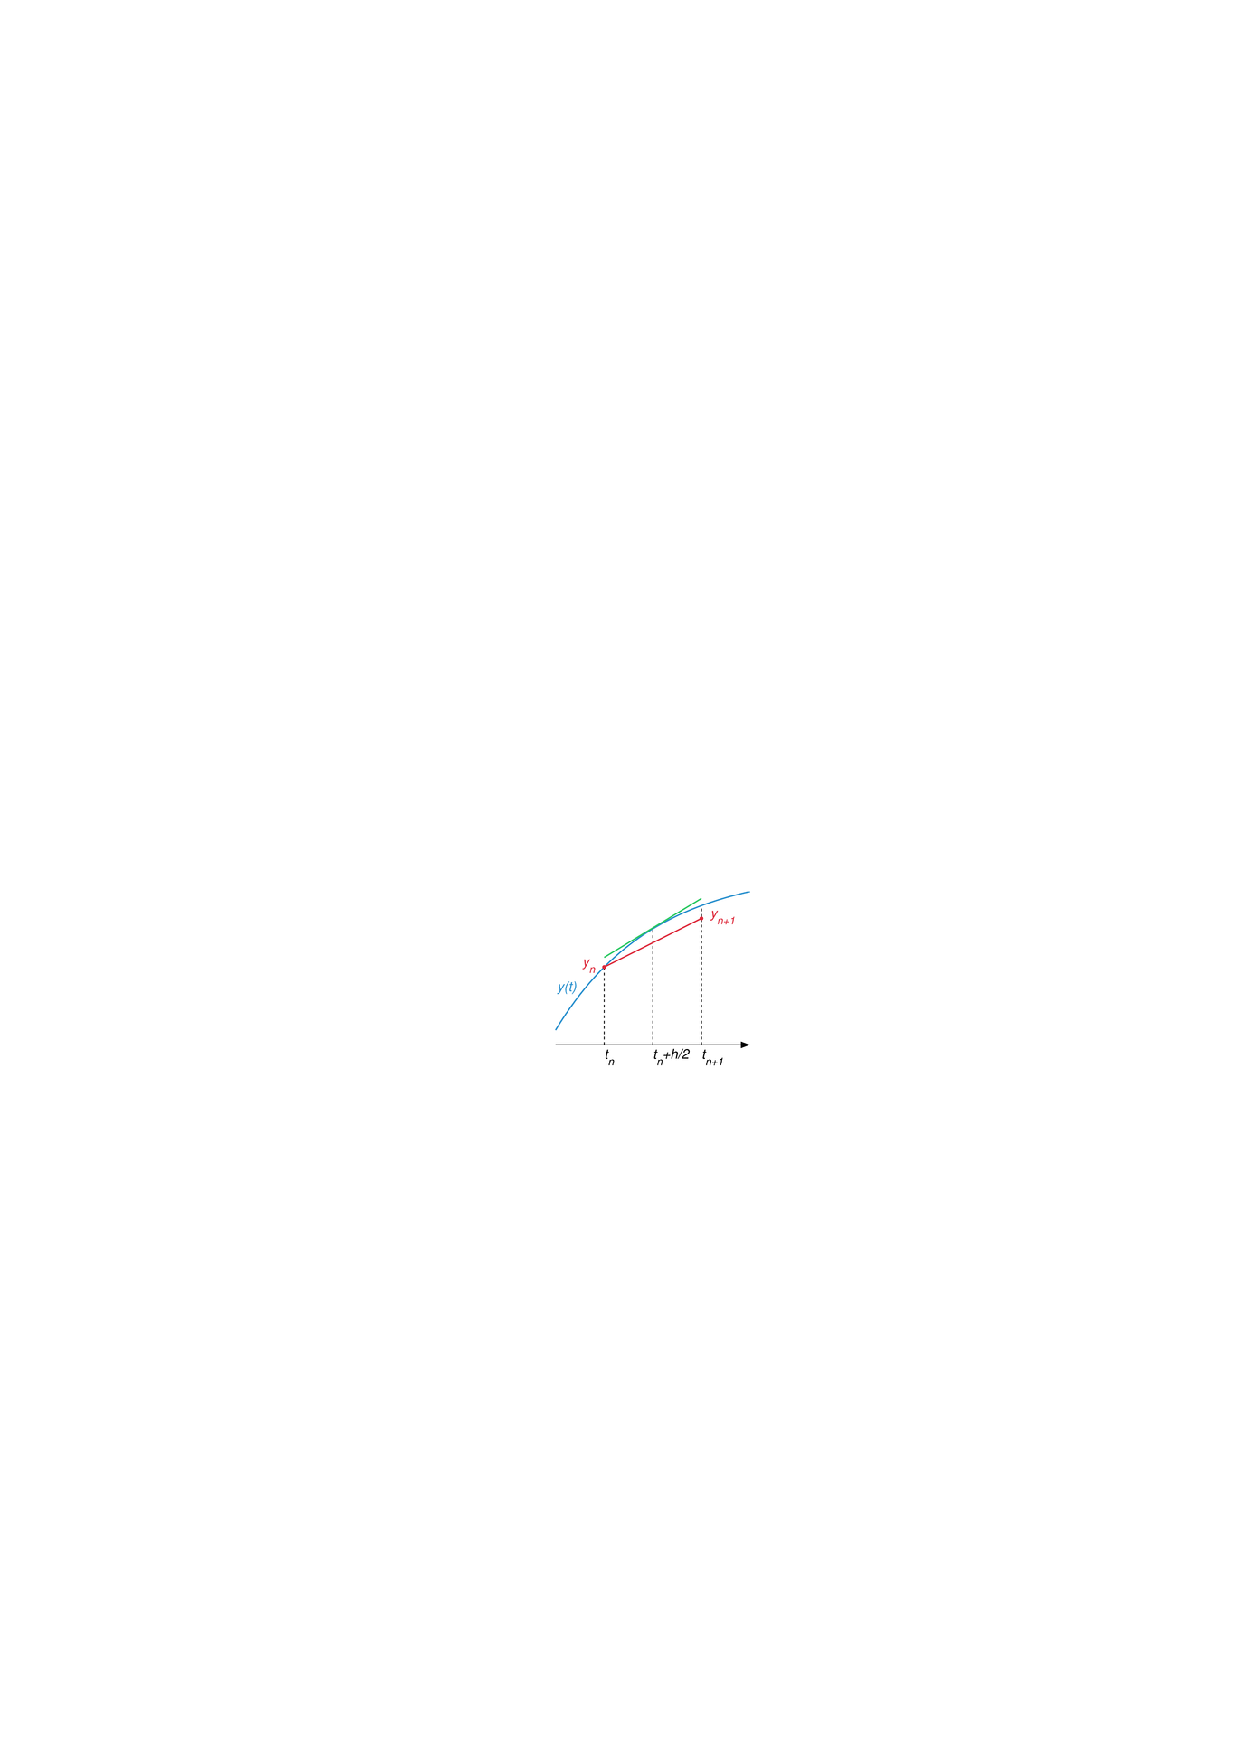
\includegraphics[width= 0.6\textwidth]{images/mittelpunkt.pdf}
\end{minipage}
\begin{minipage}{0.6\linewidth}
    \subsection{Heun-Verfahren}
    Trapez Approximation \\
    $t_k = t_0 + k  \cdot h$ \\
    $x_0 = x(0)$ \\
    $m_1 = f(t_k, x_k)$ \\
    $m_2 = f(t_k + h, x_k + hm_1)$\\
    $x_{k+1} = x_k + \frac{h}{2}(m_1 + m_1)$\\
    $e_n  \approx h^3 \qquad E_n \approx h^2$\\
\end{minipage}
\begin{minipage}{0.4\linewidth}
   % \centering
    \begin{tikzpicture}

\begin{axis} [
    clip=false,
    width=6cm, height=5cm,
    axis lines=left,
    domain=0:2.5,samples=31,
    xmin=-0.5, xmax=3.5,
    ymin=0, ymax=6,
    xticklabels={{},{},{$t_{i-1}$},{$t_i$},{}},
    yticklabels={{},{},{$f(t_{i-1},\varphi_{i-1})$},{$f(t_i,\varphi_i)$},{}},
]
    
    % Plot parabola
    \addplot[HSRBlue,mark=none] {x^2};
    \addplot[HSRBlue,mark=o,only marks] coordinates {(1,1)(2,4)};

    % Euler
    \addplot[HSRHematite,mark=none,fill=HSRHematite80,fill opacity=0.2] coordinates {(1,0)(1,1)(2,1)(2,0)(1,0)};
    \draw[HSRHematite] (axis cs:1.8,0.6) -- (axis cs:2.2,0.8) node[anchor=west] {$I_{\text{Euler}}$};    
    
    % Heun
    \addplot[HSRReed,mark=none,fill=HSRReed80,fill opacity=0.2] coordinates {(1,0)(1,1)(2,4)(2,0)(1,0)};
    \draw[HSRReed] (axis cs:1.8,2) -- (axis cs:2.2,2.2) node[anchor=west] {$I_{\text{Heun}}$};
    
\end{axis}

\end{tikzpicture}
\end{minipage}
\begin{minipage}{0.6\linewidth}
    \subsection{Runge-Kutta}
    $t_k = t_0 + k \cdot h$ \\
    $x_0 = x(0)$ \\
    $m_1 = f(t_k, x_k)$\\
    $m_2 = f(t_k + \frac{h}{2}, x_k + \frac{h}{2} m_1)$ \\
    $m_3 = f(t_k + \frac{h}{2}, x_k + \frac{h}{2} m_2)$ \\
    $m_4 = f(t_k + h, x_k + hm_3)$ \\
    $x_{k+1} = x_k + \frac{h}{6} \left(m_1 + 2m_2 + 2m_3 + m_4\right)$ \\
    $e_n \approx h^5 \qquad E_n \approx h^4$
\end{minipage}
\begin{minipage}{0.4\linewidth}
%	\centering
	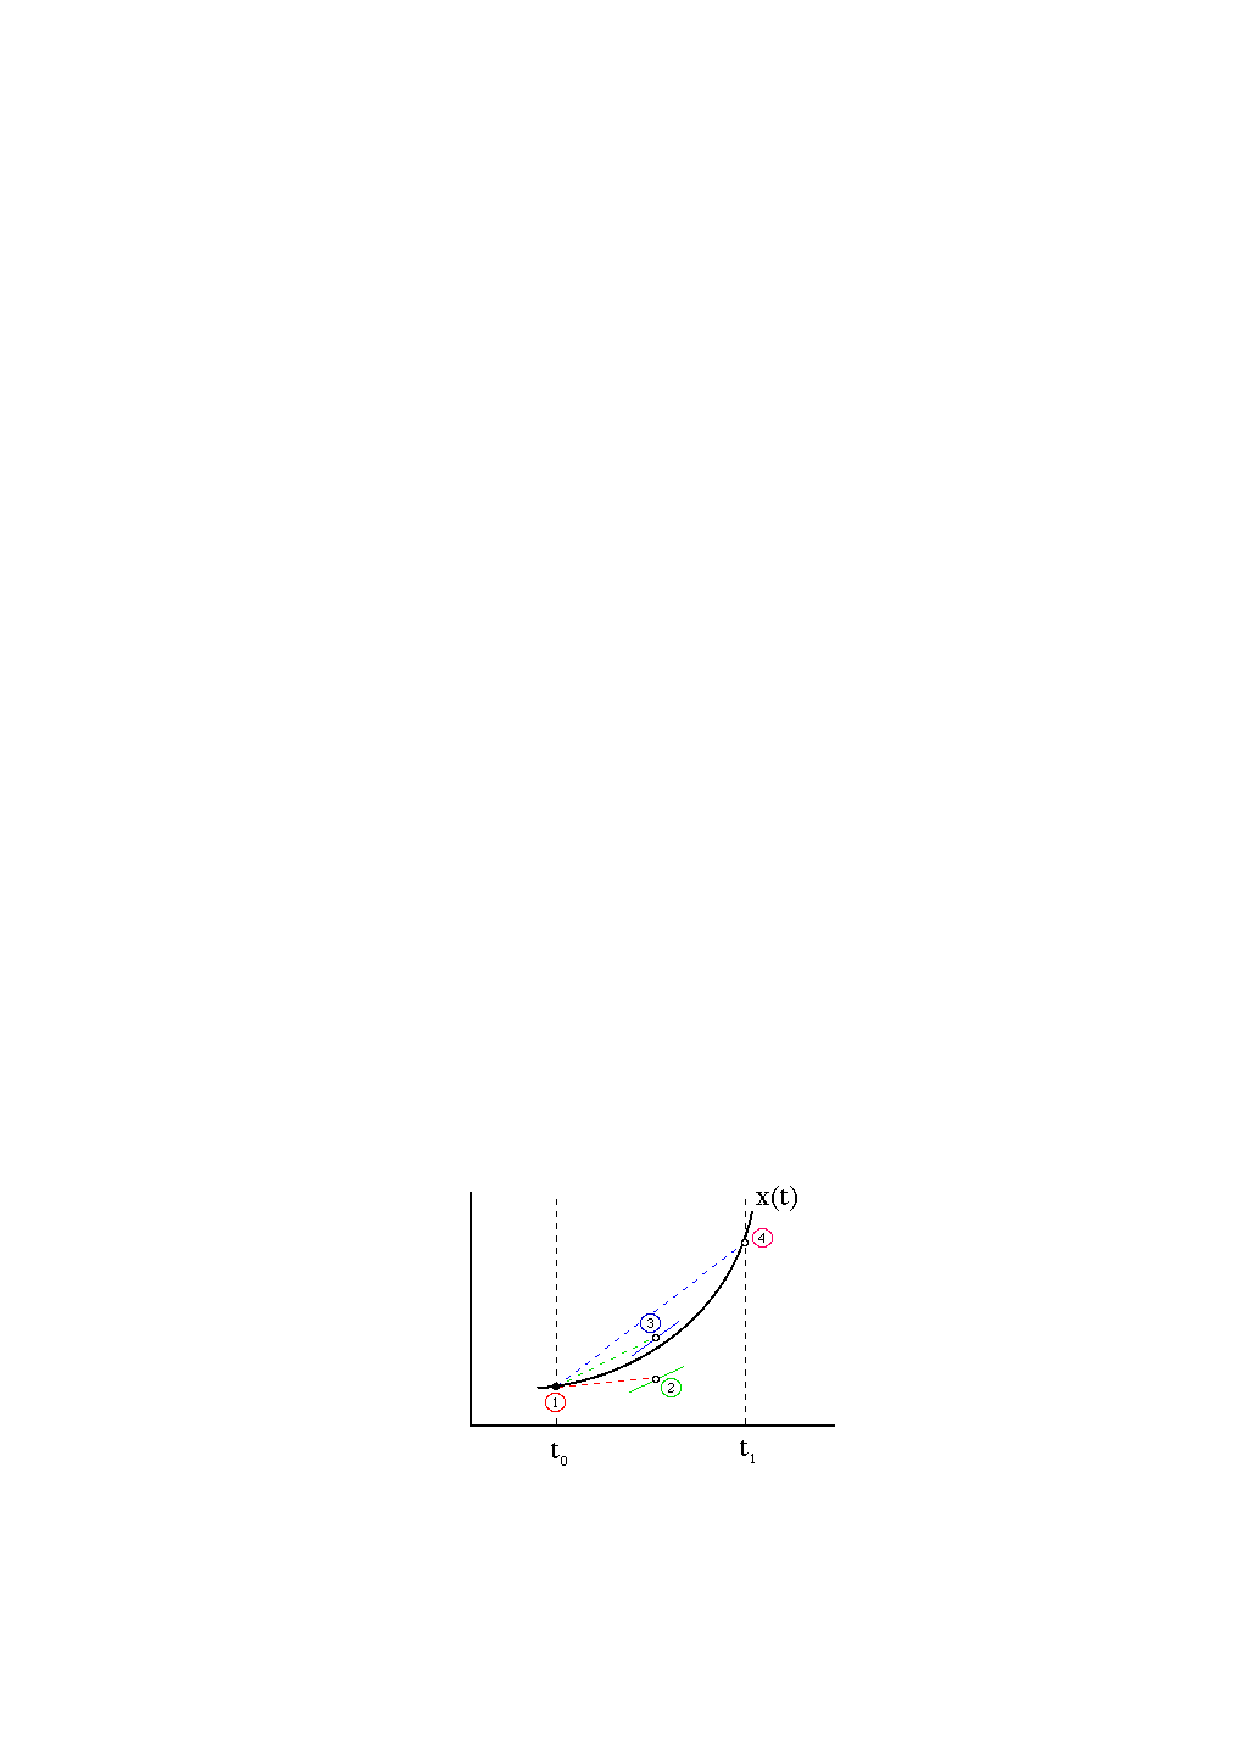
\includegraphics[width= 0.7\textwidth]{images/RK4.pdf}
\end{minipage}
\section{Dynamische Systeme}

\textbf{Fixpunkt:} $x^*:$ \hspace{1cm}$f(x^*) = 0$

\subsection{Gleichgewichtslösungen}
Die Gleichgewichtslösungen sind diejenigen Punkte, in welchen die Ableitung verschwindet:
\begin{equation*}
	\diffp{}{t}y(t) = 0
\end{equation*}
\subsection{Phasengerade und Integralkurven}
Bei der Phasengerade werden die Gleichgewichtslösungen in Funktion der Ableitung eingetragen. Dadurch kann die Stabilität eines Systems bestimmt werden. 

\subsection{Eindimensionale Syteme}
Falls $x^*$ ein \textbf{Fixpunkt} von $\dot{x} = f(x)$ ist, ist $x(t) = x^*$ eine konstante Lösung des Systems $\dot{x} = f(x)$. Der \textbf{Phasenraum} eines eindimensionalen Systems vom Typ $\dot{x} = f(x)$ is $\mathbb{R}$. Wegen des \textbf{Eindeutigkeitssatzes} hat $\dot{x} = f(x)$ für alle $0 \leq t$ das selbe Vorzeichen. Die Lösung ist daher monoton steigend, monoton fallend oder ist ein Fixpunkt. Nur für \textbf{autonome} DLG 1. Ordnung sind keine periodische Lösungen möglich.

\subsection{Lineare Stabilitätsanalyse}
\label{sec:linStab}
$\eta (t) = x(t) - x^*$ \hspace{1cm} falls $x^* \neq 0 \Rightarrow$ Taylor:\newline
$\dot{\eta} = \dot{x} = f(x) \approx f(x^*) + f'(x^*) \cdot \underbrace{(x - x^*)}_{\eta (t)}(x - x^*) = f'(x^*) \cdot \eta$ \\
$\Rightarrow \mathrm{DGL}: \dot{\eta} = \eta \cdot f'(x^*),$ \hspace{1cm} $\eta(t) = \eta(0) \cdot e^{f'(x^*)t}$ 

\begin{tabular}{ll}
	\textbf{stabil:} \quad & $f'(x^*) < 0$ \\
	\textbf{instabil:} & $f'(x^*) > 0$ \\
	\textbf{(in)stabil:} & $f'(x^*) = 0$ \\
\end{tabular}

\begin{multicols}{2}
	\subsection{Bifurkationen}
	
	\begin{equation*}
		\dot{x} = f(x,r), \quad r \in \mathbb{R}
	\end{equation*}
	
	Eine qualitative Änderung der Dynamik eines von einem Parameter $r$ abhängigen Systems, heisst Bifurkation. Die Parameterwerte von $r$ an denen diese qualitativen Änderungen erfolgen, heissen \textbf{Bifurkationspunkte} des Systems.
	\columnbreak
	\subsubsection{Saddle-Node-Bifurkation}
	Fixpunkte können durch Variation von $r$ erzeugt oder zerstört werden.
	
	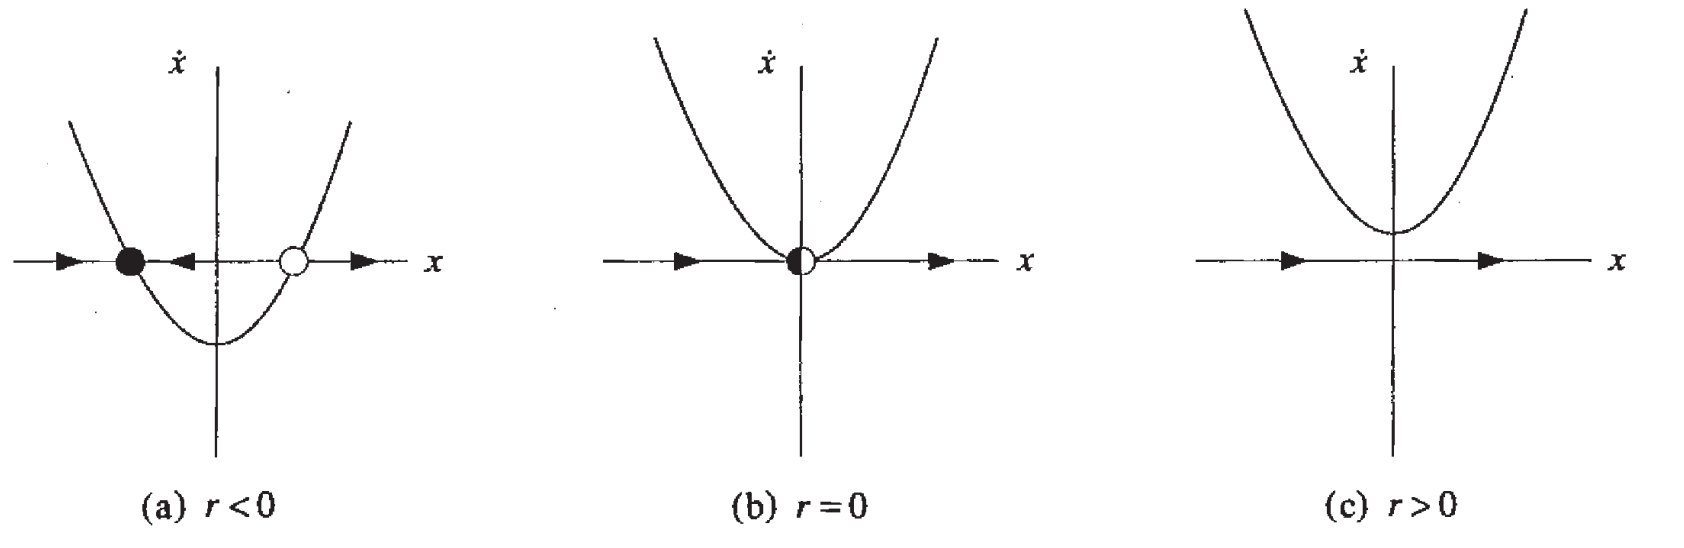
\includegraphics[width=0.5\textwidth]{./images/Saddle_Node.png}
\end{multicols}

\begin{multicols}{2}
	\subsubsection{Pitchfork-Bifurkation}
	Die Pitchfork Bifurkation ist eine Bifurkation, bei der ein Fixpunkt seine Stabilität änder und gleichzeitig zwei neue Fixpunkte entstehen. \newline \newline
	
	\textbf{superkritische Pitchfork-Bifurkation:} Man nennt diesen Typ von Bifurkation superkritisch, weil die Fixpunkte $x^* \neq 0$ nur für Parameterwerte \textbf{über} dem Bifurkationspunkt existieren, bzw. für $r >0$.
	
	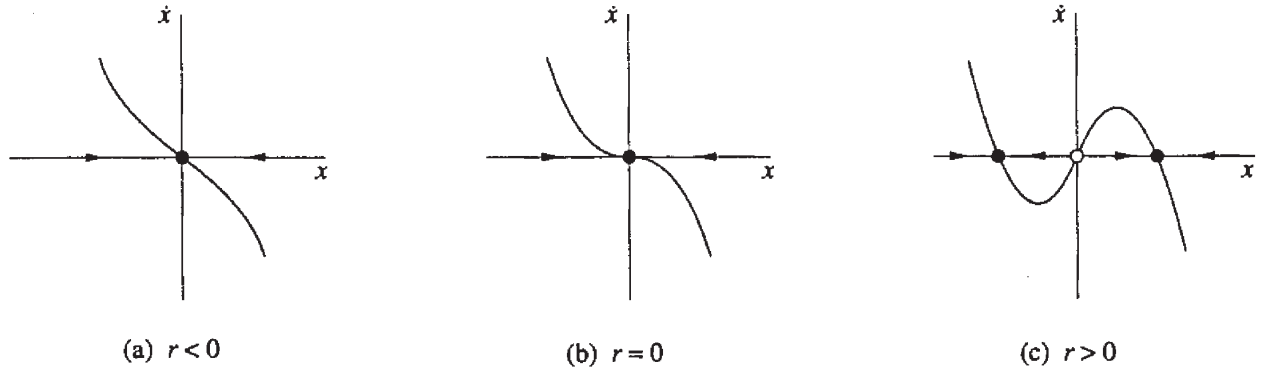
\includegraphics[width=0.5\textwidth]{./images/superkritisch.png}
	\columnbreak
	
	\textbf{subkritische Pitchfork-Bifurkation:} Man nennt diesen Typ von Bifurkation subkritisch, weil die Fixpunkte $x^* \neq 0$ nur für Parameterwerte \textbf{unter} dem Bifurkationspunkt existieren.
	
	\subsubsection{Transkritische Bifurkation}
	Bei einer transkritischen Bifurkation werden keine Fixpunkte erzeugt oder vernichtet, allerdings wird die Stabilität zweier Fixpunkte vertauscht.
\end{multicols}

\subsection{Bifurkationsdiagramm}
	Diagramm der kritischen Punkte in Abhängigkeit eines Parameters (e.g. $a$).
	
	Beispiel:
	
	\[y'=y(a-y)\]
	
\begin{tabular}{p{0.3\textwidth}p{0.3\textwidth}p{0.3\textwidth}}
	\vspace{0pt}	
	\begin{tabular}[h]{p{0.1\textwidth}p{0.2\textwidth}}
	Ausgezogen:		& Asymptotisch Stabil\\
	Gestrichelt:	& Instabil\\
	Zentrum:		& Semistabil\\
	\end{tabular}
	& 	\vspace{0pt}
		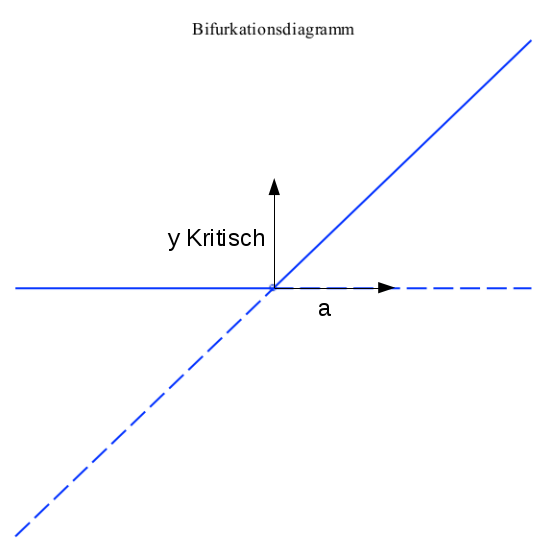
\includegraphics[width=0.3\textwidth]{images/Bifurkationsdiagramm.png}
	& 	\vspace{0pt}
		\textbf{Vorgehen:}
		\begin{tabular}[h]{p{0.02\textwidth}p{0.28\textwidth}}
		1:	& Kritische Punkte berechnen ($\dot{x} = 0$). Ergibt $x^*_k(a)$.\\
		2:	& Stabilität der Punkte berechnen (gemäss Section \ref{sec:linStab}).\\
		3:	& Kurven in Diagramm ($x^*(a)$ aufzeichnen).\\
		\end{tabular}\\
\end{tabular}

\subsection{Zweidimensionale Systeme}

\begin{tabular}{ll}
	\textbf{stabil:} & $\lvert x(t) - x^*\rvert < \epsilon \quad 0 < t < \infty$ \\
	\textbf{instabil:} & $\lvert x(t) - x^*\rvert \nless \epsilon \quad 0 < t < \infty$ \\
	\textbf{asymptotisch stabil:} & $\lim\limits_{t \to \infty} \lvert x(t) - x^*\rvert = 0$ \\
\end{tabular}

\subsubsection{Typen von Fixpunkten}

\begin{tabular}{|p{0.25\textwidth}|p{0.7\textwidth}|}
	\hline
	\textbf{Spur:} & $\tau = \mathrm{tr}(A) = a_{11} + a_{22} = \lambda_1 + \lambda_2$ \\
	\textbf{Determinante:} & $\Delta = \det(A) = a_{11}a_{22}  - a_{12}a_{21} = \lambda_1 \lambda_2$\\
	\textbf{Eigenwerte:} & $\lambda_{1,2} = \frac{1}{2} \left(\tau \pm \sqrt{\tau^2 - 4\Delta}\right)$ \\
	\hline
\end{tabular}

\begin{longtable}{|p{0.25\textwidth}|p{0.7\textwidth}|}
	\hline 
	\textbf{Eigenwerte} & \textbf{Stabilität} \endhead
	\hline
	
	\multicolumn{2}{l}{Für $\Delta > 0$ und $\tau < 0$ gilt:} \\
	
	\hline $\operatorname{Re}(\lambda_1) < 0$ und $\operatorname{Re}(\lambda_2) < 0$ & stabiler Knotenpunkt ($\tau^2 - 4 \Delta > 0$ bzw. $ \lambda_1, \lambda_2 \in \mathbb{R}$) \\
	 & stabiler Strudelpunkt ($\tau^2 - 4 \Delta < 0$ bzw. $ \lambda_1, \lambda_2 \notin \mathbb{R}$) \\
	\hline
	
	\multicolumn{2}{l}{Für $\Delta > 0$ und $\tau > 0$ gilt:}\\
	
	\hline $\operatorname{Re}(\lambda_1) > 0$ und $\operatorname{Re}(\lambda_2) > 0$ & instabiler Knotenpunkt ($\tau^2 - 4 \Delta > 0$ bzw. $ \lambda_1, \lambda_2 \in \mathbb{R}$) \\
	 & instabiler Strudelpunkt ($\tau^2 - 4 \Delta < 0$ bzw. $ \lambda_1, \lambda_2 \notin \mathbb{R}$) \\
	\hline
	
	\multicolumn{2}{l}{Für $\Delta > 0$ und $\tau = 0$ gilt:} \\
	
	\hline $\operatorname{Re}(\lambda_1) = \operatorname{Re}(\lambda_2) = 0$ & Zentrum bzw. einen elliptischen Fixpunkt\\
	\hline
	
	\multicolumn{2}{l}{Für $\Delta = 0$ gilt:} \\
	
	\hline $\lambda_1 = 0$ oder $\lambda_2 = 0$ & degeneriertes System; Fixpunkte sind nicht isoliert(bspw. ganze Gerade als Fixpunkte) \\
	\hline
	
	\multicolumn{2}{l}{Für $\Delta < 0$ gilt:} \\
	
	\hline $\lambda_1 < 0 < \lambda_2$ & Sattelpunkt (saddle point) \\
	\hline $\lambda_2 < 0 < \lambda_1$ & Sattelpunkt (saddle point) \\
	\hline
	
	\multicolumn{2}{l}{\textbf{Allgemein:}}\\
	
	\hline
	\textbf{grenzstabil:} & $\operatorname{Re}(\lambda_i) \leq 0$ für alle $\lambda_i$ \\
	\textbf{instabil:} & $\operatorname{Re}(\lambda_i) > 0$ für mind. einen Wert \\
	\textbf{asymptotisch stabil:} &$\operatorname{Re} < 0$ für alle $\lambda_i$ \\
	\hline
\end{longtable}

\subsection{Atraktorbereich und Separatrizen}
Haben wir ein autonomes System mit Anfangswertproblem. Die Gesamtheit aller Punkte des Phasenraums - die als Anfangsbedingung gewählt - zu einer Trajektorie führen, welche dann gegen einen speziellen Punkt konvergiert, heisst Atraktorbereich des Punktes. 
Die Ränder, welche diese Bereiche trennen, heissen Separatrizen. 
Im Bild sehen wir zwei Atraktorbereiche, welche durch die beiden blauen Kurven (die Separatrizen) getrennt sind. 
Startet man innerhalb der Blase, so konvergiert man gegen den Punkt (0,0) ansonsten gegen den Punkt (1,-2). 
\begin{minipage}[h!]{0.35\textwidth}
	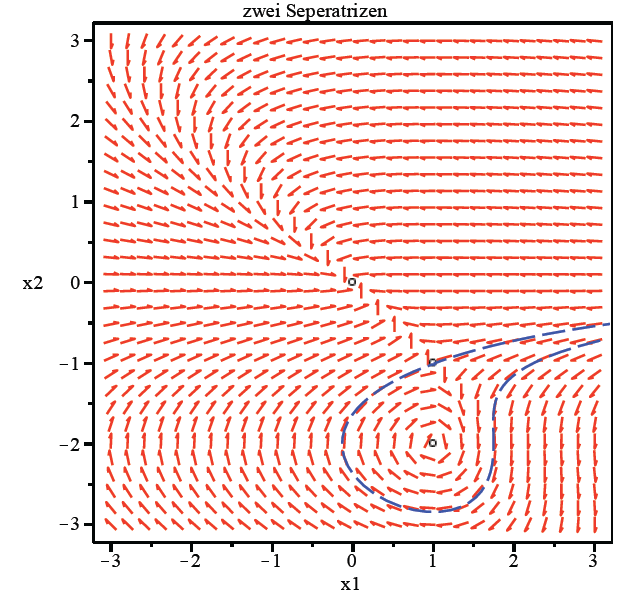
\includegraphics[width=1\textwidth]{images/Atraktorbereich.png}
\end{minipage}

\subsection{Vektorfeld und Trajektorie}
\begin{figure}[h!]
	\centering
	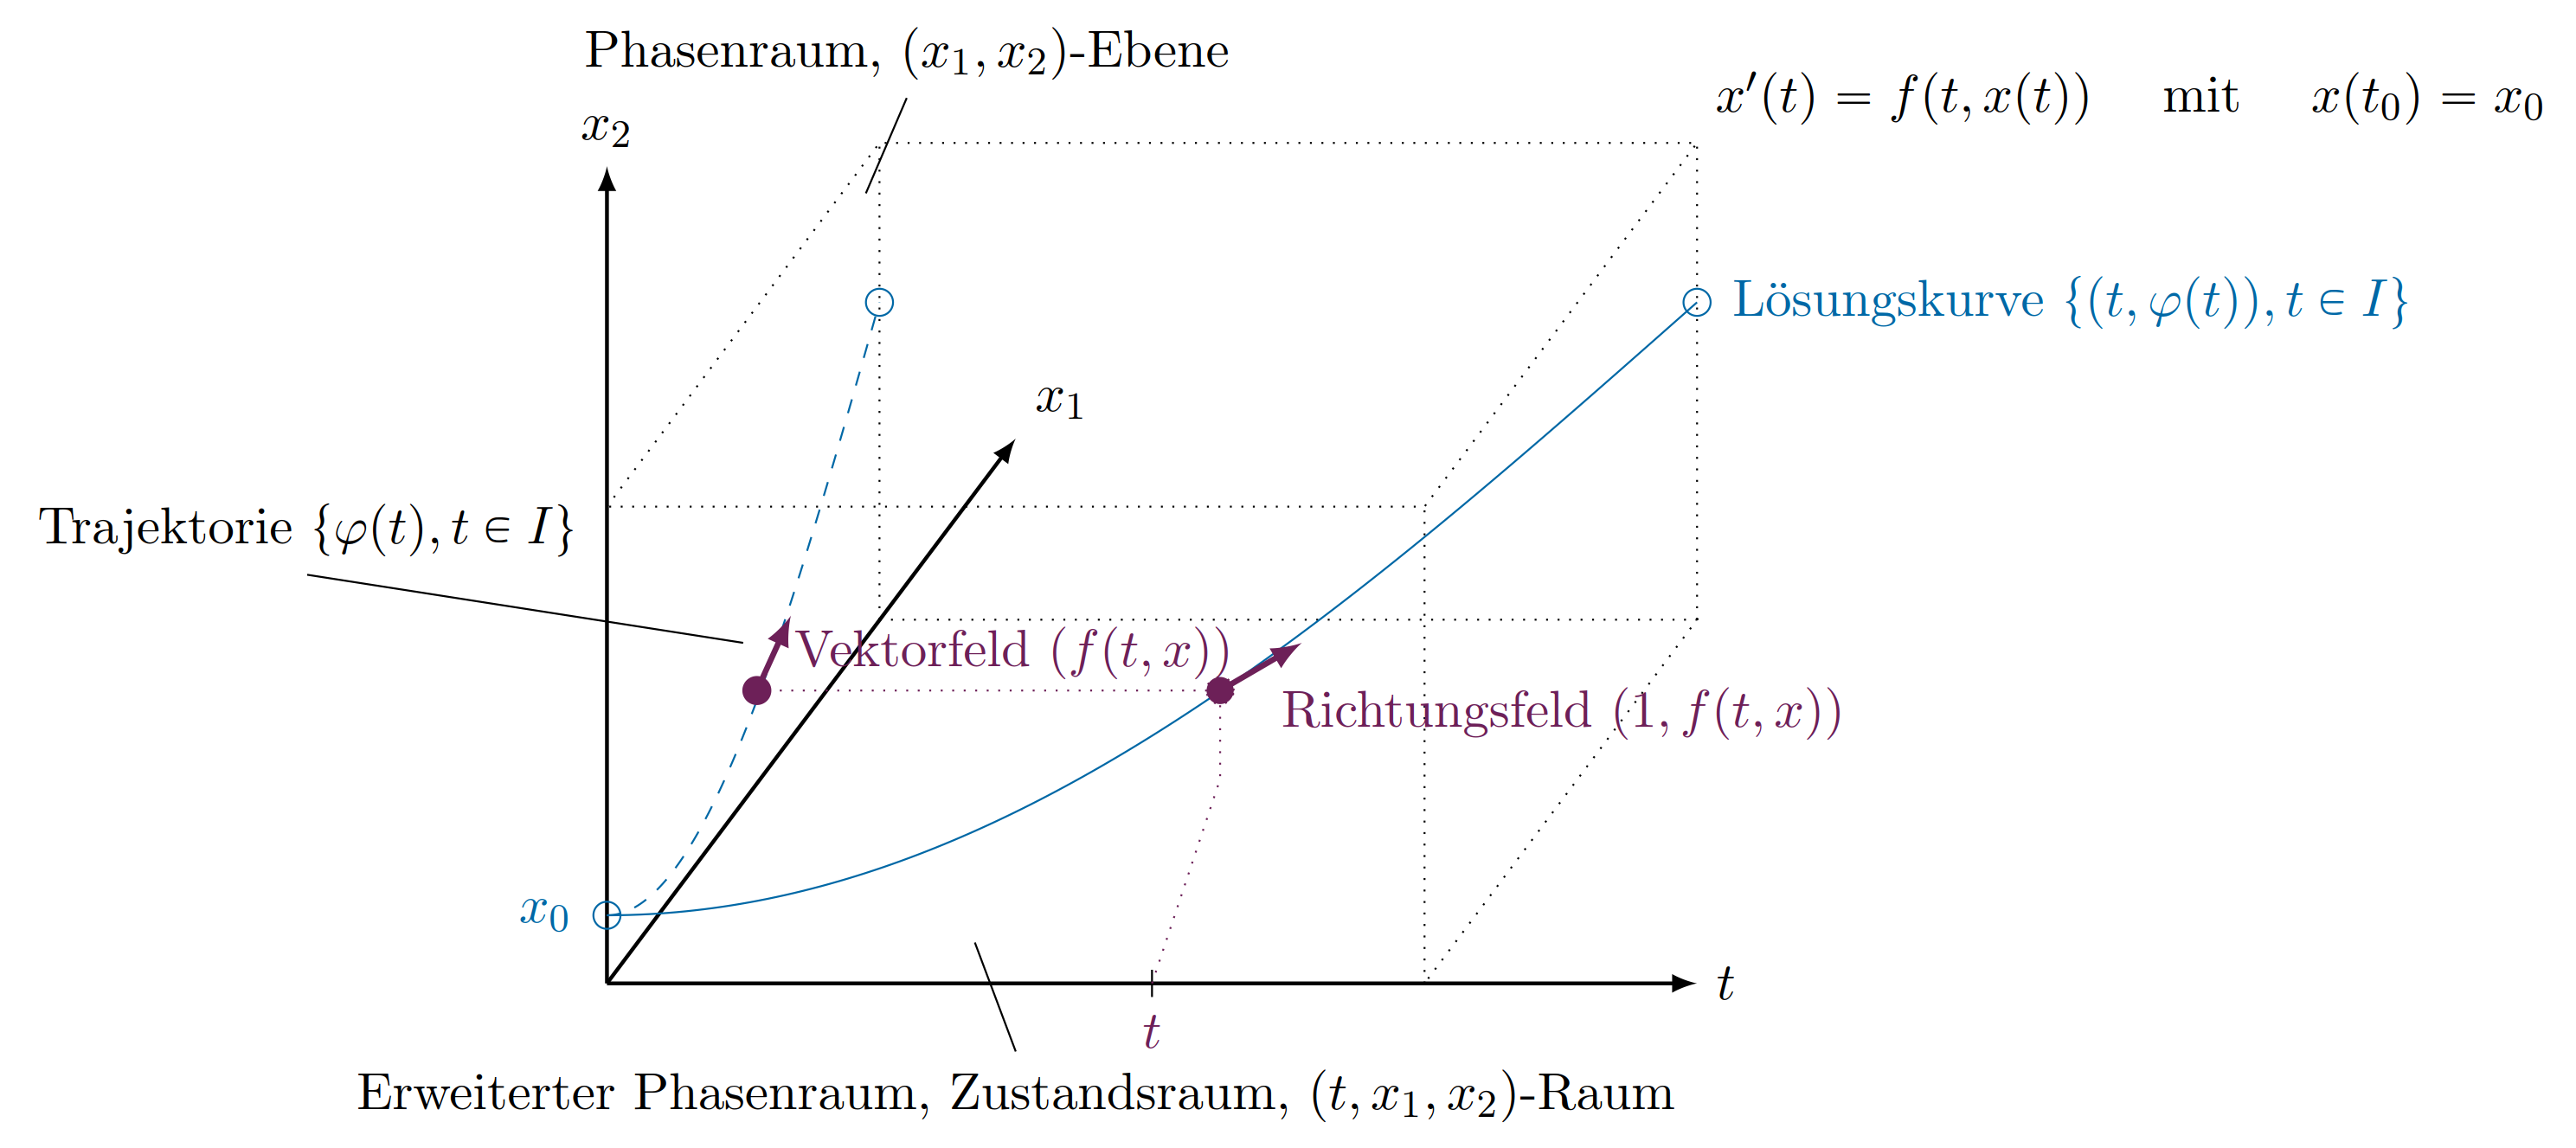
\includegraphics[width=0.8\textwidth]{./images/phasenraum.png}
\end{figure}


\subsection{Fast lineare Systeme, Jakobi-Matrix}
Ein System ist fast linear, wenn die Jacobimatrix $J_f$ regulär ist $det(J_f)\neq 0$. \\
\textbf{Robust:} Knotenpunkt, Studelpunkt, Sattelpunkt \\
\textbf{Marginal:} Zentrum, degenerierte Fälle \\ \\
1.Schritt: DGL in Form bringen:\\ 
$x'_1(t) = f_1(t) = x_2(t)$\\
$x'_2(t) = f_2(t) = -q(t)x_1(t)-p(t)x_2(t)+g(t)$\\
2.Schritt: Jacobi Matrix berechnen:\\
\begin{equation*}
	J_f(x) =    
	\begin{vmatrix} 
	        \frac{\partial f_1}{\partial x_1} & \frac{\partial f_1}{\partial x_2}\\ 
	        \frac{\partial f_2}{\partial x_1} & \frac{\partial f_2}{\partial x_2}\\   
	\end{vmatrix}
\end{equation*}
3. Schritt: Kritische Punkte berechnen (Ableitungen Null setzen...) $\rightarrow x^* = (x_{k1}^*, x_{k2}^*)$\\
4. Schritt: Jeden kritischen Punkt separat in die Jacobimatrix einsetzen\\
5. Schritt: Anschliessen für jede Jacobimatrix die Eigenwerte ausrechnen \\
6. Schritt: Stabilität nach folgender Tabelle beurteilen\\
\section{Lineare Algebra / Matrixexponential}
%TODO by Selina
-Transformationen\\
-Jordan Normalform / Berechnung mit TI89\\
-Matrixexponential 
\section{Idiotenseite}
\subsection{Dreiecksformeln}
\begin{tabular}{lll}
	& \parbox{9.5cm}{
		\textbf{Cosinussatz} \\
		$$c^2 = a^2 + b^2 - 2 \cdot a \cdot b \cdot \cos \gamma$$\\
		\textbf{Sinussatz} \\
		$$\frac{a}{\sin \alpha} = \frac{b}{\sin \beta} = \frac{c}{\sin \gamma} = 2r =
		\frac{u}{\pi}$$
		\textbf{Pythagoras beim Sinus}\\
		$$\sin^2(b)+\cos^2(b)=1 \qquad \tan(b)=\frac{\sin(b)}{\cos(b)}$$}
		
	& \parbox{8cm}{
		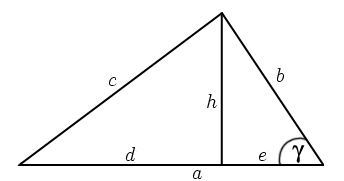
\includegraphics[width=6cm]{./idiotenseite/images/cosinussatz.png}}
\end{tabular}
\begin{center}
	\begin{multicols}{2}
		$\sin \beta = \frac ba =\frac{\text{Gegenkathete}}{\text{Hypotenuse}}$\\
		$\cos \beta = \frac ca =\frac{\text{Ankathete}}{\text{Hypotenuse}}$\\
		$\tan \beta = \frac cb =\frac{\text{Gegenkathete}}{\text{Ankathete}}$\\
		$\cot \beta = \frac cb =\frac{\text{Ankathete}}{\text{Gegenkathete}}$\\
	\end{multicols}
\end{center}

	
%\subsection{Funktionswerte für Winkelargumente}
	\begin{multicols}{4}	
	\begin{tabular}[c]{|p{0.5cm}|p{0.4cm}||p{0.5cm}|p{0.5cm}|p{0.5cm}|}
	    	\hline
			deg & rad & sin & cos & tan\\
			\hline
			0\symbol{23} & 0 & 0 & 1 & 0\\
			\hline
			30\symbol{23} & $\frac{\pi}{6}$ & $\frac{1}{2}$ & $\frac{\sqrt{3}}{2}$ &
			$\frac{\sqrt{3}}{3}$\\
			\hline
			45\symbol{23} & $\frac{\pi}{4}$ & $\frac{\sqrt{2}}{2}$ & $\frac{\sqrt{2}}{2}$
			& 1\\
			\hline
			60\symbol{23} & $\frac{\pi}{3}$ & $\frac{\sqrt{3}}{2}$ & $\frac{1}{2}$ &
			$\sqrt{3}$\\
			\hline			
	\end{tabular} \\
	
	\begin{tabular}[c]{|p{0.7cm}|p{0.7cm}||p{0.7cm}|p{0.7cm}|}
	    	\hline
			deg & rad & sin & cos\\
			\hline
			90\symbol{23} & $\frac{\pi}{2}$ & 1 & 0\\
			\hline	
			120\symbol{23} & $\frac{2\pi}{3}$ & $\frac{\sqrt{3}}{2}$ & $-\frac{1}{2}$ \\
			\hline
			135\symbol{23} & $\frac{3\pi}{4}$ & $\frac{\sqrt{2}}{2}$ & $-\frac{\sqrt{2}}{2}$\\
			\hline
			150\symbol{23} & $\frac{5\pi}{6}$ & $\frac{1}{2}$ & $-\frac{\sqrt{3}}{2}$\\
			\hline
	\end{tabular} \\
	
	\begin{tabular}[c]{|p{0.7cm}|p{0.7cm}||p{0.7cm}|p{0.7cm}|}
	  	\hline
		deg & rad & sin & cos\\
		\hline
		180\symbol{23} & $\pi$ & 0 & -1\\
		\hline	
		210\symbol{23} & $\frac{7\pi}{6}$ & $-\frac{1}{2}$ & $-\frac{\sqrt{3}}{2}$\\
		\hline
		225\symbol{23} & $\frac{5\pi}{4}$ & $-\frac{\sqrt{2}}{2}$ & $-\frac{\sqrt{2}}{2}$\\
		\hline
		240\symbol{23} & $\frac{4\pi}{3}$ & $-\frac{\sqrt{3}}{2}$ & $-\frac{1}{2}$\\
		\hline
	\end{tabular} \\
	
	\begin{tabular}[c]{|p{0.7cm}|p{0.7cm}||p{0.7cm}|p{0.7cm}|}
    	\hline
		deg & rad & sin & cos\\
		\hline
		270\symbol{23} & $\frac{3\pi}{2}$ & -1 & 0\\
		\hline	
		300\symbol{23} & $\frac{5\pi}{3}$ & $-\frac{\sqrt{3}}{2}$ & $\frac{1}{2}$\\
		\hline
		315\symbol{23} & $\frac{7\pi}{4}$ & $-\frac{\sqrt{2}}{2}$ & $\frac{\sqrt{2}}{2}$\\
		\hline
		330\symbol{23} & $\frac{11\pi}{6}$ & $-\frac{1}{2}$ & $\frac{\sqrt{3}}{2}$\\
		\hline
	\end{tabular}					
\end{multicols}

\begin{minipage}{13cm}
	\subsection{Periodizität}
	$\cos(a+k\cdot2\pi)=\cos(a) \qquad \sin(a+k\cdot2\pi)=\sin(a) \qquad
	(k \in \mathbb{Z})$
	\subsection{Quadrantenbeziehungen}
	\begin{tabbing}
    	xxxxxxxxxxxxxxxxxxxxxxxxxxxxxxxxxx \= \kill
	  	$\sin(-a)=-\sin(a)$ \> $\cos(-a)=\cos(a)$\\
		$\sin(\pi - a)=\sin(a)$ \> $\cos(\pi - a)=-\cos(a)$\\
		$\sin(\pi + a)=-\sin(a)$ \> $\cos(\pi +a)=-\cos(a)$\\
		$\sin\left(\frac{\pi}{2}-a \right)=\sin\left(\frac{\pi}{2}+a \right)=\cos(a)$ \>
		$\cos\left(\frac{\pi}{2}-a \right)=-\cos\left(\frac{\pi}{2}+a \right)=\sin(a)$  
    \end{tabbing}
\end{minipage}
\begin{minipage}{5cm}
	

\subsection{Ableitungen}

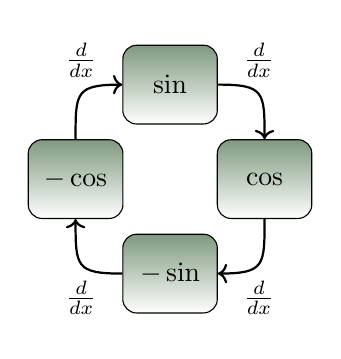
\begin{tikzpicture}
	[	inner sep = 2mm,
		sin/.style={rectangle,minimum width=1.2cm,minimum height=1cm,rounded corners=5pt,draw=black,top color=green!20!black!50},
		abl/.style={rectangle}
	]
	\node at (1.2,0) (sin1) [sin] {$\sin$};
	\node at (0,-1.2) (cos2) [sin] {$-\cos$};
	\node at (1.2,-2.4) (sin2) [sin] {$-\sin$};
	\node at (2.4,-1.2) (cos1) [sin] {$\cos$};
	
	\draw[thick,black,->] (sin1.east) .. controls +(right:0.6cm) and +(up:0.6cm) ..  (cos1.north)
	node [pos=0.5,above](abl) {$\frac{d}{dx}$};
	\draw[thick,black,->] (cos1.south) .. controls +(down:0.6cm) and +(right:0.6cm) .. (sin2.east)
	node [pos=0.5,below](abl) {$\frac{d}{dx}$};
	\draw[thick,black,->] (sin2.west) .. controls +(left:0.6cm) and +(down:0.6cm) .. (cos2.south)
	node [pos=0.5,below](abl) {$\frac{d}{dx}$};
	\draw[thick,black,->] (cos2.north) .. controls +(up:0.6cm) and +(left:0.6cm) .. (sin1.west)
	node [pos=0.5,above](abl) {$\frac{d}{dx}$};
\end{tikzpicture}
\end{minipage}
\begin{multicols}{2}
	\subsection{Additionstheoreme}
	$\sin(a \pm b)=\sin(a) \cdot \cos(b) \pm \cos(a) \cdot \sin(b)$\\
	$\cos(a \pm b)=\cos(a) \cdot \cos(b) \mp \sin(a) \cdot \sin(b)$\\	
	$\tan(a \pm b)=\dfrac{\tan(a) \pm \tan(b)}{1 \mp \tan(a) \cdot \tan(b)}$
%	\columnbreak 
	
	\subsection{Doppel- und Halbwinkel}	
	$\sin(2a)=2\sin(a)\cos(a)$\\
	$\cos(2a)=\cos^2(a)-\sin^2(a)=2\cos^2(a)-1=1-2\sin^2(a)$\\
	$\cos^2 \left(\frac{a}{2}\right)=\frac{1+\cos(a)}{2} \qquad
	\sin^2 \left(\dfrac{a}{2}\right)=\frac{1-\cos(a)}{2}$ \\
	$\tan\frac{\alpha}{2} = \frac{\sin \alpha}{1 + \cos \alpha} = \frac{1- \cos \alpha}{\sin \alpha} = \sqrt{\frac{1 - \cos \alpha}{1 + \cos \alpha}}$ \\
	$\tan 2 \alpha = \frac{2 \tan \alpha}{1 - \tan^2 \alpha} = \frac{2}{\cot \alpha - \tan \alpha}$ \\
%\end{multicols}
%\begin{multicols}{2}
	\subsection{Produkte}
		$\sin(a)\sin(b)=\frac{1}{2}(\cos(a-b)-\cos(a+b))$\\
		$\cos(a)\cos(b)=\frac{1}{2}(\cos(a-b)+\cos(a+b))$\\
		$\sin(a)\cos(b)=\frac{1}{2}(\sin(a-b)+\sin(a+b))$\\
	\subsection{Euler-Formeln} 

	$\sin(x) = \frac{1}{2j} \left(e^{jx} - e^{-jx}\right) \qquad
	\cos(x) = \frac{1}{2} \left(e^{jx} + e^{-jx}\right)$ \\
	$e^{x+jy} = e^x \cdot e^{jy} = e^x \cdot \left(\cos(y) + j\sin(y)\right)$ \\
	$e^{j\pi} = e^{-j\pi} = -1$ \\
%	\columnbreak
	
	\subsection{Summe und Differenz}
		$\sin(a)+\sin(b)=2 \cdot \sin \left(\frac{a+b}{2}\right) \cdot
		\cos\left(\frac{a-b}{2}\right)$\\
		$\sin(a)-\sin(b)=2 \cdot \sin \left(\frac{a-b}{2}\right) \cdot
		\cos\left(\frac{a+b}{2}\right)$\\
		$\cos(a)+\cos(b)=2 \cdot \cos \left(\frac{a+b}{2}\right) \cdot
		\cos\left(\frac{a-b}{2}\right)$\\
		$\cos(a)-\cos(b)=-2 \cdot \sin \left(\frac{a+b}{2}\right) \cdot
		\sin\left(\frac{a-b}{2}\right)$\\
		$\tan(a) \pm \tan(b)=\dfrac{\sin(a \pm b)}{\cos(a)\cos(b)}$\\
\end{multicols}

\begin{sidewaystable}
\subsection{Einige unbestimmte Integrale\formelbuch{1074}}
\label{unbestimmte_integrale}
\begin{tabular}{|p{12cm}|p{12cm}|}
  \hline
  
    $ \int dx=x+C $ &
     $ \int{x^\alpha}dx=\frac{x^{\alpha+1}}{\alpha+1}+C,\ x \epsilon \mathbb
    R ^+,\ \alpha \epsilon \mathbb R \backslash \{ -1 \} $ \\\hline
     $ \int{\frac{1}{x}}dx=\ln \left| x \right| + C,\ x\neq0 $ &
     $ \int{e^x}dx=e^x+C $ \\\hline
     $ \int{a^x}dx=\frac{a^x}{\ln{a}}+C,\ a \epsilon \mathbb 
    R^+\backslash\{1\} $ &
     $ \int{ \sin{x}} dx = -\cos{x} + C $ \\\hline
     $ \int{\cos{x}} dx = \sin{x} + C $ &
     $ \int{\frac{dx}{\sin^2x}}=-\cot{x}+C,\ x\neq k\pi\ \mathrm{mit}\ k
    \epsilon \mathbb Z $ \\\hline
     $ \int{\frac{dx}{\cos^2x}}=\tan{x}+C,\ x\neq\frac{\pi}{2}+k\pi\
    \mathrm{mit} k \epsilon \mathbb Z $ & 
    
    %10. :
     $ \int{\sinh{x}}dx = \cosh{x}+C $ \\ \hline
     $ \int{\cosh{x}}dx = \sinh{x}+C $ &
     $ \int{\frac{dx}{\sinh^2x}}=-\coth{x}+C,\ x\neq0 $ \\\hline
     $ \int{\frac{dx}{\cosh^2x}}=\tanh{x}+C $ &
     $ \int{\frac{dx}{ax+b}} = \frac{1}{a}\ln \left|ax + b\right| + C,\
    a\neq 0,x\neq-\frac{b}{a} $ \\\hline
     $ \int{\frac{dx}{a^2x^2+b^2}}=\frac{1}{ab}\arctan{\frac{a}{b}x}+C,\
    a\neq0,\ b\neq0 $ &
     $
    \int{\frac{dx}{a^2x^2-b^2}}=\frac{1}{2ab}\ln{\left|\frac{ax-b}{ax+b}\right|}+C,\
    a\neq0,\ b\neq0,\ x\neq\frac{b}{a},\ x\neq-\frac{b}{a} $ \\\hline
     $
    \int{\sqrt{a^2x^2+b^2}}dx=\frac{x}{2}\sqrt{a^2x^2+b^2}+\frac{b^2}{2a}\ln{(ax+\sqrt{a^2x^2+b^2})}+C,\
    a\neq0,\ b\neq0 $ &
     $
    \int{\sqrt{a^2x^2-b^2}}dx=\frac{x}{2}\sqrt{a^2x^2-b^2}-\frac{b^2}{2a}\ln\left|ax+\sqrt{a^2x^2-b^2}\right|+C,\
    a\neq0,\ b\neq0,a^2x^2\geqq b^2$ \\\hline
     $
    \int\sqrt{b^2-a^2x^2}dx=\frac{x}{2}\sqrt{b^2-a^2x^2}+\frac{b^2}{2a}\arcsin\frac{a}{b}x+C,\
    a\neq0,\ b\neq0,\ a^2x^2\leqq b^2 $ &
    %20.:
     $
    \int\frac{dx}{\sqrt{a^2x^2-b^2}}=\frac{1}{a}\ln(ax+\sqrt{a^2x^2+b^2})+C,\
    a\neq0,\ b\neq0 $ \\\hline
     $
    \int\frac{dx}{\sqrt{a^2x^2-b^2}}=\frac{1}{a}\ln\left|ax+\sqrt{a^2x^2-b^2}\right|+C,\
    a\neq0,\ b\neq0,\ a^2x^2>b^2 $ &
     $ \int\frac{dx}{\sqrt{b^2-a^2x^2}}=\frac{1}{a}\arcsin\frac{a}{b}x+C,\
    a\neq0,\ b\neq0,\ a^2x^2<b^2 $ \\\hline
     Die Integrale $\int\frac{dx}{X}, \int\sqrt{X}dx,
    \int\frac{dx}{\sqrt{X}}$ mit $X=ax^2+2bx+c,\ a\neq0 $ werden durch 
    die Umformung $X=a(x+\frac{b}{a})^2+(c-\frac{b^2}{a}) $ und die
    Substitution $ t=x+\frac{b}{a} $ in die oberen 4 Zeilen
    transformiert. & $ \int\frac{xdx}{X}=\frac{1}{2a}\ln\left|X\right|-\frac{b}{a}\int\frac{dx}{X},\
    a\neq0,\ X=ax^2+2bx+c $ \\\hline
     $ \int\sin^2axdx=\frac{x}{2}-\frac{1}{4a}\cdot\sin2ax+C,\ a\neq0 $ &
     $ \int\cos^2axdx=\frac{x}{2}+\frac{1}{4a}\cdot\sin2ax+C,\ a\neq0 $ \\\hline
     $ \int\sin^naxdx=-\frac{sin^{n-1}ax\cdot\cos
    ax}{na}+\frac{n-1}{n}\int\sin^{n-2}axdx,\ n \epsilon \mathbb N,\ a\neq0 $ &
     $ \int\cos^naxdx=\frac{\cos^{n-1}ax\cdot\sin
    ax}{na}+\frac{n-1}{n}\int\cos^{n-2}axdx,\ n\epsilon \mathbb N,\ a\neq0 $
    \\\hline
     $ \int\frac{dx}{\sin ax} =
    \frac{1}{a}\ln\left|\tan\frac{ax}{2}\right|+C,\ a\neq0,\ x\neq
    k\frac{\pi}{a}\ \mathrm{mit}\ k\epsilon\mathbb Z$ &
    %30.:
     $ \int\frac{dx}{\cos
    ax}=\frac{1}{a}\ln\left|\tan(\frac{ax}{2}+\frac{\pi}{4})\right|+C,\ a\neq0,\
    x\neq\frac{\pi}{2a}+k\frac{\pi}{a}\ \mathrm{mit}\ k\epsilon\mathbb Z $
    \\\hline
     $\int\tan axdx=-\frac{1}{a}\ln\left|\cos ax\right|+C,\ a\neq0,\
    x\neq\frac{\pi}{2a}+k\frac{\pi}{a} \mathrm{mit}\ k\epsilon\mathbb Z$ &
     $\int\cot axdx=\frac{1}{a}\ln\left|\sin ax\right|+C,\ a\neq0,\ x\neq
    k\frac{\pi}{a} \mathrm{mit} k\epsilon\mathbb Z $ \\ \hline
     $ \int x^n\sin axdx=-\frac{x^n}{a}\cos ax+\frac{n}{a}\int x^{n-1}\cos
    axdx,\ n\epsilon\mathbb N,\ a\neq0 $ &
    $ \int x^n\cos axdx=\frac{x^n}{a}\sin ax-\frac{n}{a}\int x^{n-1}\sin
    axdx,\ n\epsilon\mathbb N,\ a\neq0 $ \\ \hline
     $ \int x^ne^{ax}dx=\frac{1}{a}x^ne^{ax}-\frac{n}{a}\int
    x^{n-1}e^{ax}dx,\ n\epsilon\mathbb N,\ a\neq0 $ &
     $ \int e^{ax}\sin bxdx=\frac{e^{ax}}{a^2+b^2}(a\sin bx-b\cos bx)+C,\
    a\neq0,\ b\neq0 $  \\ \hline
     $ \int e^{ax}\cos bxdx=\frac{e^{ax}}{a^2+b^2}(a\cos bx + b\sin bx)+C,\
    a\neq0,\ b\neq0 $ &
     $ \int\ln x dx = x(\ln x-1)+C,\ x\epsilon\mathbb R^+ $ \\ \hline
     $ \int x^\alpha \cdot \ln xdx =
    \frac{x^{\alpha+1}}{(\alpha+1)^2}\lbrack(\alpha+1)\ln x-1\rbrack + C,\
    x\epsilon\mathbb R^+,\ \alpha\epsilon\mathbb R\backslash\{-1\} $ & \\ \hline
    %FF1 Seite 496
    
\end{tabular}
\end{sidewaystable}
\end{document}
